% Journal manuscript, Control Engineering Practice (Elsevier, elsarticle 5p, 20-page limit).
% Build: make -C papers/cep pdf; limits: make -C papers/cep check.
% Grounded draft, branch docs/cep-grounded-draft (2026-11-03). Every number comes from a script and
% configs/camera_100.toml (Appendix A); results that need hand-labelled crystals are marked \pending{}.
% Every changed scientific claim is listed for author approval in papers/cep/CLAIM_CHANGES.md.
\documentclass[5p,authoryear]{elsarticle}

\usepackage[T1]{fontenc}
\usepackage{graphicx}
\usepackage{booktabs}
\usepackage{array}
\usepackage[hyphens,obeyspaces,spaces]{url}
\Urlmuskip=0mu plus 1mu
\usepackage{amsmath,amssymb}
\usepackage{subcaption}
\usepackage{xcolor}
\usepackage[hidelinks]{hyperref}

% Figures: the generated folder (papers/cep/figures/) first, the current optics figures as fallback.
\graphicspath{{figures/}{../../docs/optics/figures/}}
\journal{Control Engineering Practice}
\setlength{\emergencystretch}{2em}
\tolerance=2000
\newcommand{\tabfont}{\footnotesize\setlength{\tabcolsep}{3pt}}

% Units and references used throughout the sections.
\newcommand{\um}{\textmu m}
\newcommand{\umpx}{\textmu m/px}
\newcommand{\secref}[1]{\S\,\ref{#1}}
\newcommand{\figref}[1]{Figure~\ref{#1}}
\newcommand{\tabref}[1]{Table~\ref{#1}}
\DeclareUrlCommand\code{\urlstyle{tt}}% breakable code and paths
% Results that wait on hand-labelled crystals or site checks.
\newcommand{\pending}[1]{\textcolor{red}{[PENDING: #1]}}
\newcommand{\orcid}[1]{\texorpdfstring{\,\href{https://orcid.org/#1}{\textsuperscript{\textsf{iD}}}}{}}

\begin{document}
\begin{frontmatter}

\title{Towards in-line crystal sizing through the sight glass of an industrial sugar seed pan: pixel scale, depth
of field and detector failure modes}

% Authors, order and ORCIDs from docs/paper/CREDIT.md. All: Slovak University of Technology in Bratislava.
\author[STU]{Marek Wadinger\orcid{0000-0002-0167-6331}\corref{cor}}
\ead{marek.wadinger@stuba.sk}
\author[STU]{Patrik Val\'abek\orcid{0009-0006-9201-3651}}
\author[STU]{Erika Pl\v{s}i\v{c}\'ik Pavlovi\v{c}ov\'a\orcid{0000-0003-4335-8347}}
\author[STU]{Ananya Lohani\orcid{0009-0006-8079-2475}}
\author[STU]{Mari\'an Choma\orcid{0009-0001-1956-0003}}
\author[STU]{Radoslav Paulen\orcid{0000-0002-1599-2634}}
\cortext[cor]{Corresponding author.}
\affiliation[STU]{organization={Slovak University of Technology in Bratislava}, city={Bratislava},
country={Slovakia}}

\begin{abstract}
An in-line crystal-size signal from the seed pan would let a soft sensor track crystal growth in sugar boiling, yet we
found no reported in-line size measurement through the sight glass of an industrial sugar pan. We examine what
the camera installed at the seed-pan sight glass of Slovensk\'e cukrovary, Sere\v{d}, can measure. It
is an analogue monochrome PAL CCD camera behind a 35~mm lens on an extension tube of about 60~mm. We model the chain
from CCD cell through 13.5~MHz digitisation to 1080p screen recordings and tag every input with its source. The
1080p clips are screen recordings of the PAL picture, stretched $2.677 \times 1.875$, and add no resolution. At the focused plane a clip pixel spans $1.464 \times 1.913$~\um{} and a PAL sample
$3.92 \times 3.59$~\um, each within about $\pm 10$\,\% at 95\,\%, dominated by the tube length. At F/1.6 the
in-focus slice is $\pm 9.4$~\um. Within it, the mean depth correction of sizes is at most 0.013\,\%, and a
single-component size prior cannot tell front from back: 99.6--99.9\,\% of off-focus detections receive
$p_\mathrm{near} = 0.500 \pm 0.002$. Two classical detectors return size distributions set by their area window
or seed spacing, not by the crystals. Microscope photographs of a seed-pan run show median crystal chords growing
from 29~\um{} to 483~\um{} within two hours of seeding. We define a
validation against hand-labelled crystals, whose results are pending, and show that a growth-curve calibration of the
scale needs such an independent size reference. Open scripts regenerate every number.
\end{abstract}

% CEP: 3-5 highlights of <= 85 characters, submitted as the separate file highlights.txt (CEP guide); they are not
% typeset here, because elsarticle's highlights environment adds a page that counts against the 20-page limit.

\begin{keyword}
crystal-size distribution \sep sight-glass imaging \sep sugar crystallization \sep depth of field \sep measurement
uncertainty \sep soft sensor
\end{keyword}

\end{frontmatter}

% Section 1 of manuscript v0.2 (docs/paper/manuscript.md), converted without changes to claims or numbers.
\section{Introduction}\label{sec:intro}

\subsection{What the operator needs to see}\label{sec:intro-need}

Industrial sucrose production runs as a sequence of evaporative-cooling crystallization ``strikes'' in vacuum pans. A
typical white-sugar plant operates a three-massecuite scheme --- A-, B-, and C-product --- each of which is charged
with purified syrup, concentrated to the meta-stable supersaturated state, \textbf{seeded} with a small mass of milled
sugar or magma, and then run for \textbf{three to four hours} while supersaturation is held in the growth region by
controlled vapour-pressure decrease \citep{Bubnik1995,Asadi2006}. Throughout the strike, the operator must intervene
with sweetwater additions, vacuum and temperature setpoints, and timing of cuts and discharges. The two parameters
that ultimately matter to the plant are the \textbf{mean aperture (MA)} and the \textbf{coefficient of variation (CV)}
of the discharged crystal-size distribution: MA drives downstream classification, CV controls centrifuge efficiency
and the recoverable molasses fraction. A strike that lands on the wrong MA or with excessive CV must be reworked at
substantial energy and yield cost.

Without a calibrated, real-time view of the in-vessel CSD, operator interventions rely on indirect proxies ---
conductivity, refractive index, boiling-point elevation --- that are coupled to CSD only through plant-specific
heuristics. \textbf{A reliable, non-invasive, in-line crystal-size measurement is among the most-requested unsolved
sensor problems in industrial crystallization} \citep{Nagy2013,Simon2015}.

\subsection{Why the dominant instruments fall short}\label{sec:intro-instruments}

Four families of measurement principle dominate the literature on in-line CSD monitoring; each has well-documented
limitations.

\paragraph{Probe-based optical instruments} Mettler-Toledo's \emph{Focused Beam Reflectance Measurement} (FBRM) scans
a laser through the slurry and infers a chord-length distribution from back-scattered pulses
\citep{Worlitschek2003,Heath2002}. FBRM has become a \emph{de facto} research standard but suffers from three issues
for sugar use: (i) the chord-length-to-size inversion is geometrically ill-posed and biases the recovered CSD by
15--40\,\% depending on particle shape \citep{Czapla2010}; (ii) the optical window must be kept clean against viscous
massecuite, a heavy maintenance burden at sugar-pan temperatures and concentrations; (iii) each FBRM probe costs
50--150~kEUR and requires dedicated data acquisition. The companion \emph{Particle Vision Microscopy} (PVM) probe
produces real in-line images but no calibrated size --- sizes must be hand-measured on extracted frames --- and its
very shallow depth-of-field limits useful observation to a thin slice immediately in front of the probe
\citep{Wynn2003,Eggers2008}.

\paragraph{Indirect spectroscopic and acoustic methods} NIR and Raman spectroscopy can track \emph{solute
concentration} and \emph{supersaturation} in real time \citep{Borissova2009}; acoustic-emission methods correlate
ultrasonic absorption with loading. None of these \emph{measure} CSD; they all require calibration against an
independent CSD reference, inheriting that reference's biases.

\paragraph{Off-line laser diffraction and sieving} The industrial gold standards --- Malvern Mastersizer, sieve
cascades --- deliver a calibrated CSD but only after sampling, dilution, and laboratory transport. The shortest
practical cycle is 30--60 minutes, far slower than the operator-decision time scale during the latter half of a
strike.

\paragraph{Through-sight-glass image analysis} A \emph{retrofit-free} alternative is to install a camera looking
through an existing sight glass. Hardware investment is a few hundred Euro; no in-vessel modification is required.
Academic and industrial groups have demonstrated the approach for pharmaceutical crystallization
\citep{Larsen2007,Borchert2014}, with recent work exploiting CNNs
for detection and shape classification \citep{Salami2021}. Yet \textbf{published through-sight-glass approaches share
two persistent weaknesses}:
\begin{enumerate}
\item Pixel-to-millimetre \textbf{calibration is treated as a prerequisite, not part of the inference}. Calibration
is accomplished by inserting a physical scale target --- a stage micrometer, engraved reticle, or reference crystal
--- into the slurry or line of sight. This is an intrusive operation requiring process shutdown and re-assembly. It
is typically performed once at install time and treated as static, even though installations drift mechanically and
thermally.
\item The \textbf{depth-of-field structure of the lens} is universally ignored. Through a sight glass, the slurry is
a three-dimensional volume; crystals at different depths project to different metric scales and with different
defocus levels. The standard approach is to apply a single scale to every detection --- accepting either a sampling
bias (sharpness thresholding) or a sizing bias (no correction).
\end{enumerate}

\subsection{The methodological building blocks already exist}\label{sec:intro-blocks}

The components needed to address both weaknesses are mature in the optics, computer-vision, and
crystallization-engineering literatures. Our contribution is their composition into an end-to-end pipeline, not their
individual derivation:
\begin{itemize}
\item \textbf{Geometric optics through a sight glass:} Gaussian thin-lens model
(\citealp[Ch.~5]{Hecht2017}; \citealp[Ch.~4]{BornWolf1999}), flat-glass refractive shift
(\citealp[\S\,5.6]{Hecht2017}; exact polynomial form in \citealp{Agrawal2012}).
\item \textbf{Defocus and depth-from-defocus:} geometric circle-of-confusion \citep{Pentland1987,Pertuz2013},
Gaussian-PSF sharpness fall-off \citep{SubbaraoSurya1994}, Sum-Modified-Laplacian focus measure
\citep{NayarNakagawa1994}.
\item \textbf{Front/back ambiguity for circular apertures:} \citet{Zhou2011} establish that circular-aperture defocus
is symmetric in reciprocal object distance, breaking sign disambiguation from blur alone.
\item \textbf{Crystal-growth kinetics:} McCabe's $\Delta L$ law \citep{McCabe1929,RandolphLarson1988} predicts
linear-in-time growth at fixed supersaturation, providing the cross-batch invariant we exploit for self-validation.
\end{itemize}

\subsection{Problem statement and research questions}\label{sec:rq}

Given a fixed camera looking through a sight glass into the vessel, with sensor pitch known, lens partially
characterised, glass standard known but thickness only estimated, and an archive of complete batches with known
start-of-strike timestamps, deliver: (a) a per-frame estimate of the CSD that \textbf{accounts for the
depth-of-field structure of the lens}, (b) uncertainty quantification on every numerical output, (c) a soft-sensor
read-out of time-since-graining validated against the wall-clock reference --- using only the video archive, batch
start timestamps, and documented optics, without any in-line scale target or hardware modification.

The work is organised around four research questions:
\begin{description}
\item[RQ1.] Does the thin-lens model yield a self-consistent pixel-to-millimetre mapping under the documented lens
parameters, and to what precision are the uncertain parameters (extension tube, focus setting) bounded by in-scene
evidence alone? (\secref{sec:optics})
\item[RQ2.] Does the empirical per-pixel sharpness distribution agree with the geometric-optics Gaussian-PSF
prediction, and to what precision? (\secref{sec:defocus})
\item[RQ3.] Can the front/back depth ambiguity of circular-aperture defocus be broken using the focal-plane
apparent-size distribution as a \textbf{single-component} Bayesian prior under a homogeneous-slurry assumption?
(\S\S\,\ref{sec:detection}--\ref{sec:sizing})
\item[RQ4.] Across multiple boiling-pan strikes, does the per-batch median apparent crystal size as a function of
time-into-strike collapse to a single curve, and can this collapse identify the lens-stack parameters that would
otherwise be hardware-measured? (\secref{sec:growth} outlook)
\end{description}

\subsection{The pipeline at a glance}\label{sec:glance}

The full pipeline composes six stages. \figref{fig:pipeline} shows the dataflow.

\begin{figure*}
\centering
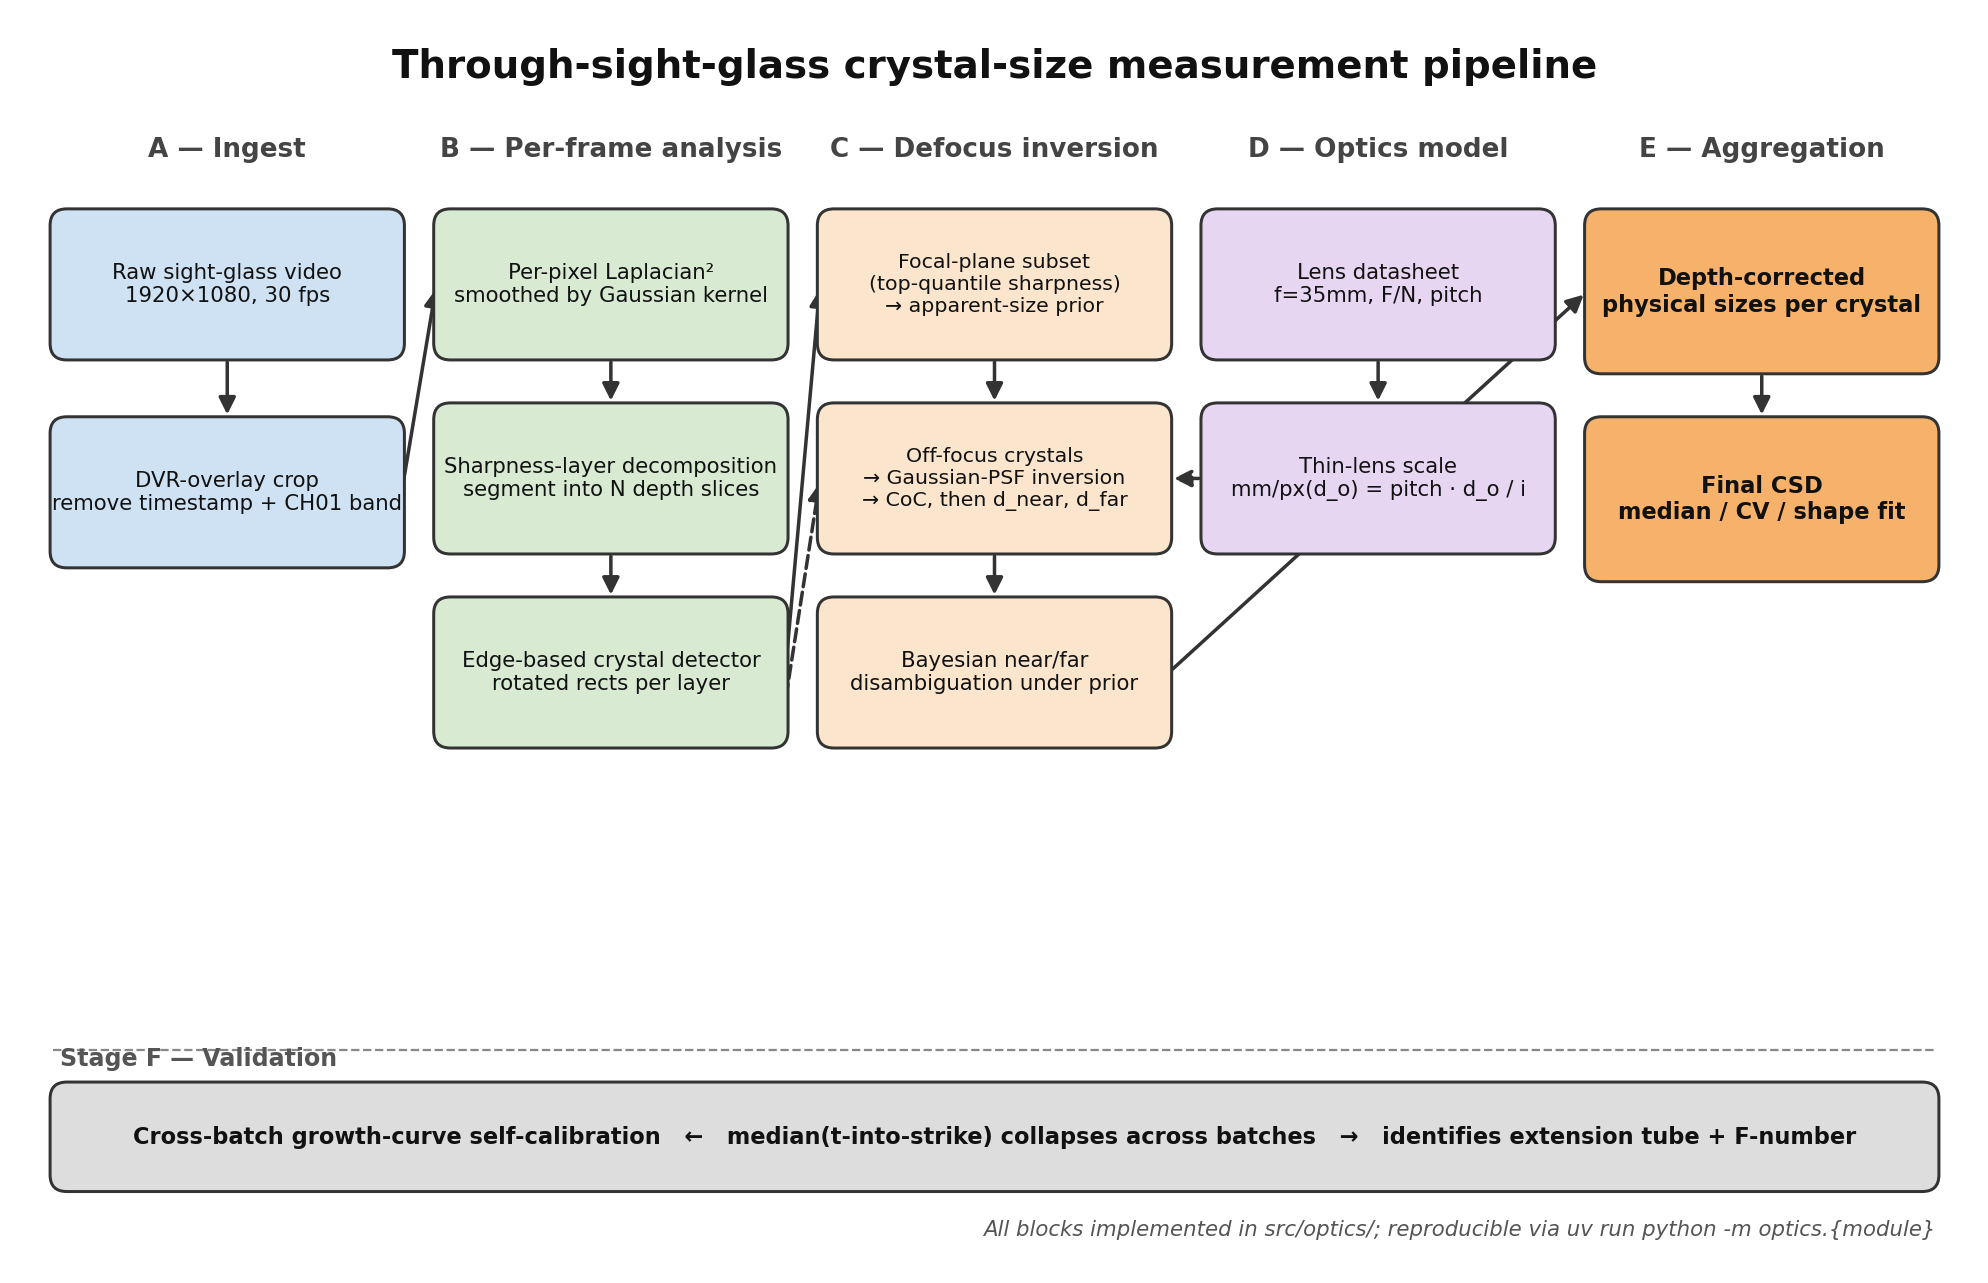
\includegraphics[width=0.75\textwidth]{13_pipeline}
\caption{\textbf{What is the full pipeline, end to end?} Stages A--E (top row) compose the forward measurement: raw
video $\rightarrow$ DVR-overlay crop $\rightarrow$ per-frame sharpness analysis $\rightarrow$ per-crystal defocus
inversion $\rightarrow$ thin-lens optics scale $\rightarrow$ aggregated CSD. Stage F (bottom bar) is the cross-batch
growth-curve self-validation discussed in \secref{sec:growth}. Every block is implemented as a reproducible Python
module under \texttt{src/optics/} and is exercised by the case-study run of
\S\S\,\ref{sec:optics}--\ref{sec:csd}.}\label{fig:pipeline}
\end{figure*}

\subsection{Contributions}\label{sec:contrib}

\begin{enumerate}
\item \textbf{A complete, open-source pipeline} that delivers calibrated CSD from raw through-sight-glass video by
integrating geometric optics, defocus analysis, Bayesian disambiguation, and growth-curve self-validation. MIT
licence, code at \emph{(URL)}.
\item \textbf{A single-component depth-aware sizing framework} that breaks the front/back defocus ambiguity using the
focal-plane apparent-size distribution as prior, under a documented homogeneous-slurry assumption that admits a
built-in self-consistency check (\secref{sec:sizing}).
\item \textbf{A quantitative treatment of detector--depth interaction}, including the explicit conditions under which
the disambiguation regime is operationally resolvable and the discriminability ceiling imposed by edge-based
detectors (\secref{sec:selectivity}).
\item \textbf{A validated industrial case study} at Slovensk\'e cukrovary, Sere\v{d}, demonstrating the pipeline on
archived video with a complete numerical audit trail.
\item \textbf{An honest failure-mode discussion} including the DVR-overlay contamination we encountered, the loss of
disambiguation power when the detector's depth selectivity is too narrow, and the refractive limits of the paraxial
sight-glass model.
\end{enumerate}

% Section 2 of manuscript v0.2 (docs/paper/manuscript.md), converted without changes to claims or numbers.
\section{Hardware and recording setup}\label{sec:hardware}

\subsection{Plant and vessel}\label{sec:plant}

Camera 100 is installed at the Slovensk\'e cukrovary sugar plant in Sere\v{d}, Slovakia, on the \textbf{seed pan}:
the graining vacuum pan, designated ZRA in the plant control system (Slovak \emph{o\v{c}kovac\'i varostroj};
Slovensk\'e cukrovary plant Q\&A, 2026-08-12; DeltaV ``Udaje ZRA'' screen; \citealp{SlovenskeCukrovary2026};
English--Slovak glossary in Appendix~\ref{app:glossary}). The seed pan is seeded with milled-sugar slurry
(\emph{mikroo\v{c}ko}) and produces the seed massecuite (\emph{o\v{c}kovacia cukrovina}) that is dosed into the A
vacuum pans, where the product is boiled (operator A.~Fedor, pers.\ comm., 2026-11-03); the C stage is likewise
started from seed massecuite (plant Q\&A). The seed slurry's crystal-size distribution is independently characterised
by laser-diffraction granulometry (Mastersizer, 2-propanol dispersant; see \secref{sec:csd} preface and
\citealp{Mastersizer2025}) with $D[3;2] = 3.95$~\um, $D[4;3] = 8.71$~\um{} and
$\mathrm{Dv}(10) / \mathrm{Dv}(50) / \mathrm{Dv}(90) = 1.56 / 6.81 / 18.5$~\um. Vessel-level dimensions, agitation
regime, and operating temperature of the seed pan have not yet been independently audited and are deferred to a
follow-up revision; the camera-side hardware (\secref{sec:camera}) is operator-verified.

The seed pan is mechanically stirred (stirrer current tag EI1004) in normal operation, which is the physical basis on
which we invoke the homogeneous-slurry assumption of \secref{sec:homog}: the stirred massecuite continually refreshes
the slab actually imaged through the sight glass (\secref{sec:slab}), so the millimetre-thin slice is a
near-representative sample of the bulk population. A stage-specific audit of the recirculation rate vs.\ residence
time is on the follow-up list.

The camera observes the slurry through a circular borosilicate sight glass marked \code{DIN 8902}, mounted on an
8-bolt PN10 flange (\O150~mm / DN150, 20~mm thick, both measured on site 2026-09-07). The lens stack is horizontal,
with transmitted illumination from an LED inside the vessel on the opposite side of the slurry. Full hardware audit
and photographs are in the project's lens documentation (\code{docs/lens/README.md}).

\subsection{Camera and lens}\label{sec:camera}

The camera is a \textbf{Hanwha Vision HCB-6000}, an analogue HD box camera with a 1/2.8\,in progressive-scan CMOS
sensor (Sony IMX307/IMX327 die, identified from the datasheet total-pixel count $1945 \times 1097$;
$5.57 \times 3.13$~mm active area, $1920 \times 1080$~px, 2.9~\um{} pitch, 30~fps, AHD/TVI/CVI/CVBS-PAL output). The
lens is a \textbf{Fujinon HF35HA-1B}, a C-mount machine-vision lens with $f = 35$~mm, F-number range F/1.6 -- F/22,
image-format 2/3\,in (\O~11~mm circle), minimum object distance 0.25~m, back focal distance 15.03~mm in air, manual
iris with lock screws. Operator measurement on site (2026-06-15, corrected 2026-09-07) yielded an extension tube of
$\boldsymbol{e = 60}$~\textbf{mm} between the lens C-mount thread and the camera body, an F-number setting of
\textbf{F/1.6} (wide open), and a lens-front-to-glass air gap of $\boldsymbol{a = 20}$~\textbf{mm}. These numbers
together fix the working distance $d_\mathrm{focus} = 55.1$~mm and the scale 1.66~\umpx{} (\secref{sec:thinlens});
they are used throughout this paper.

\begin{quote}
\textbf{Revision note (2026-09-07).} Geometry and all detector outputs (CSD, KPI tables) in this manuscript were
rerun at the measured $e = 60$~mm / $t = 20$~mm / $a = 20$~mm. The dent-sharpness figure (\figref{fig:dents}) and
its $c = 5.8$~\um{} calibration predate the correction; its generating script is not in the repository.
\end{quote}

\subsection{Recording protocol and frame conditioning}\label{sec:recording}

The case-study video is \code{2026-02-05 10-36-32.mp4} (1568 frames, 30~fps, $1920 \times 1080$~px). The recording
carries \textbf{two distinct sources of frame contamination}, both of which inject artificially sharp edges that
overwhelm any per-pixel sharpness statistic computed on the raw frame (\secref{sec:empirical}):
\begin{enumerate}
\item \textbf{A burnt-in DVR overlay} --- a digital \code{YYYY-MM-DD HH:MM:SS} timestamp band in the top
${\sim}45$ rows and a \code{CH01} channel label in the bottom ${\sim}100$ rows. These are \emph{infinitely sharp
digital glyphs}.
\item \textbf{Analogue-aspect black bars} --- the leftmost ${\sim}40$ columns and the rightmost ${\sim}55$ columns
are pitch black (the analogue capture chain pads 4:3 source into a 16:9 frame). The transition between the black
bar and the live image produces a Laplacian$^2$ value of ${\sim}110$ (vs ${\sim}10$ for typical crystal-edge pixels)
--- an order of magnitude above any real signal.
\end{enumerate}

Both are removed by a single conservative frame crop: \code{CropBox(top=55, bottom=120, left=50, right=70)} from
\code{optics.video_io}. The cropped frame retains $1800 \times 905$~px $\approx 78$\,\% of the original frame area.
The crop box is one parameter; tune per recording if the DVR layout or analogue-aspect padding differs.

\figref{fig:frames} shows the raw and cropped first frame side by side. Every figure below uses the cropped variant.

\begin{figure}
\centering
\begin{subfigure}{\columnwidth}
\centering
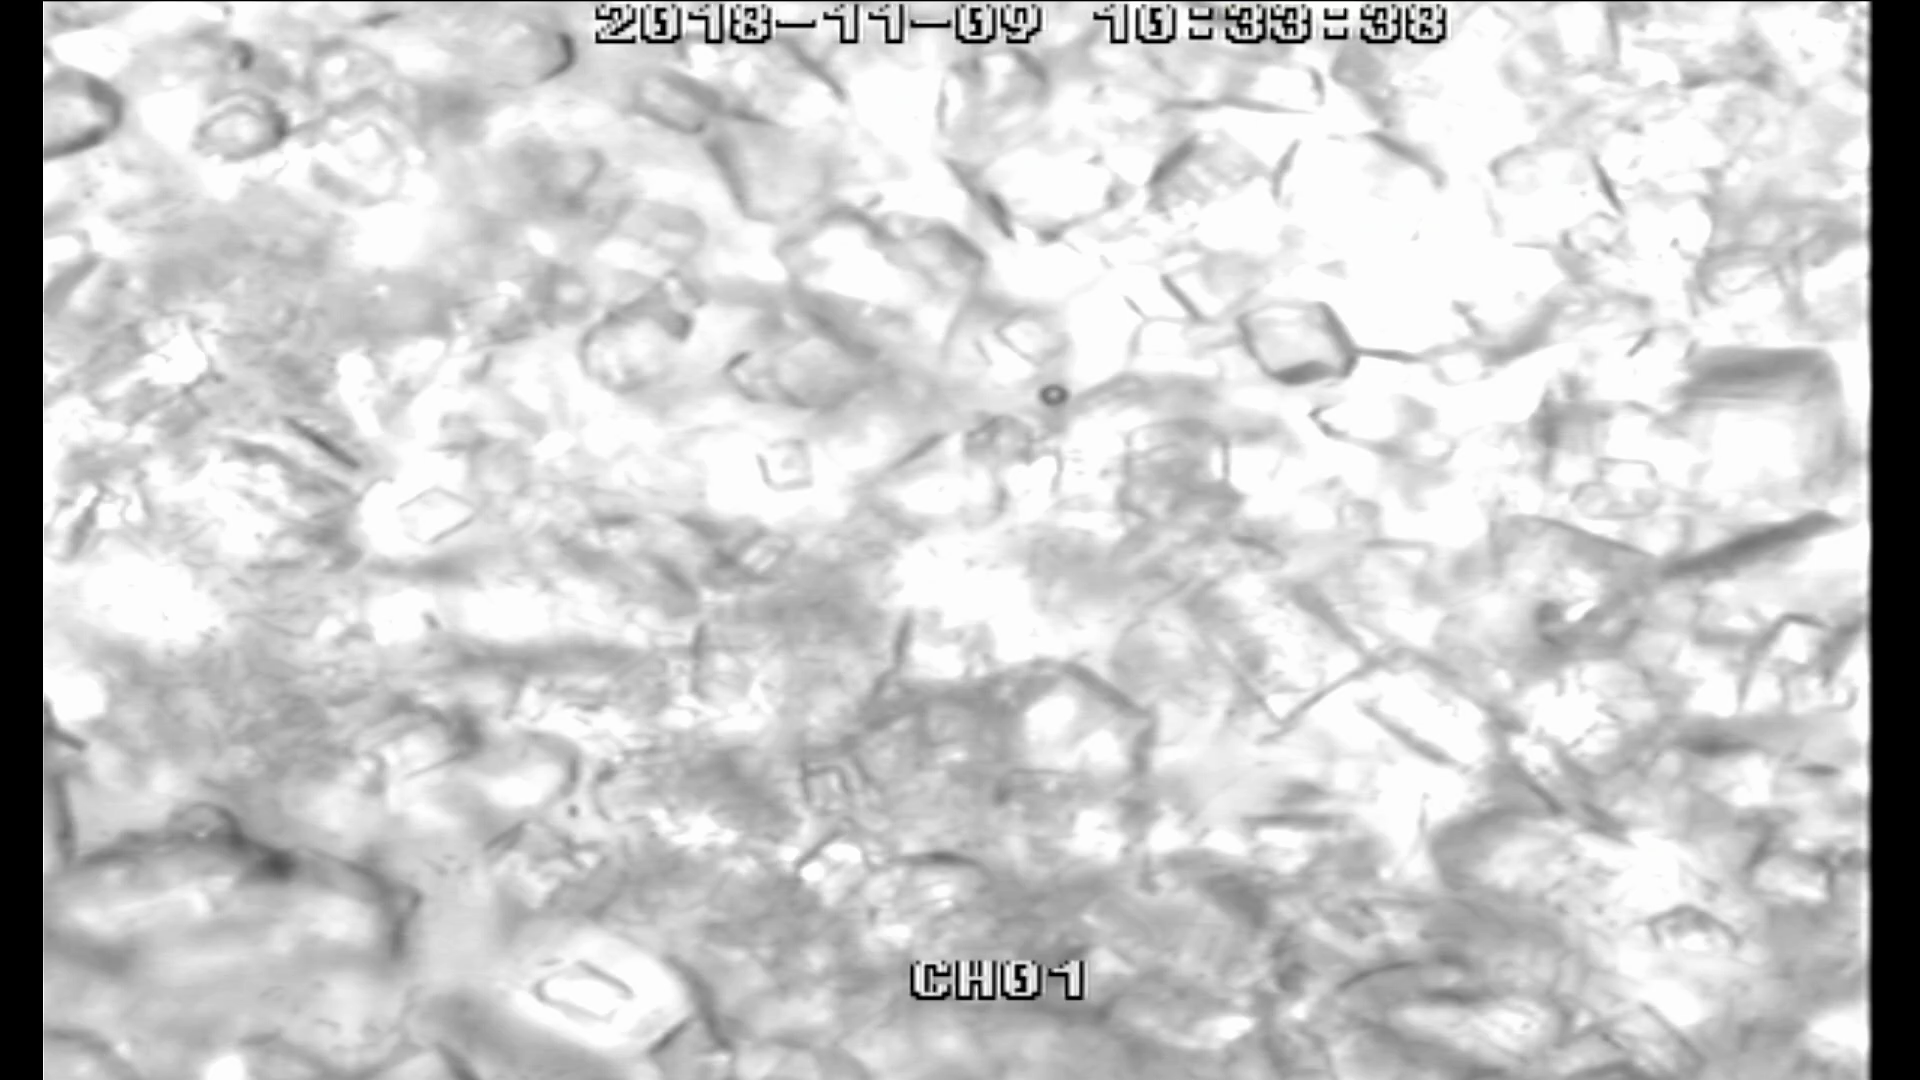
\includegraphics[width=\linewidth]{00_first_frame}
\caption{Raw first frame, $1920 \times 1080$. Top: DVR timestamp band. Bottom: \texttt{CH01} label. Left \& right:
analogue-aspect black bars.}\label{fig:frames-raw}
\end{subfigure}

\medskip
\begin{subfigure}{\columnwidth}
\centering
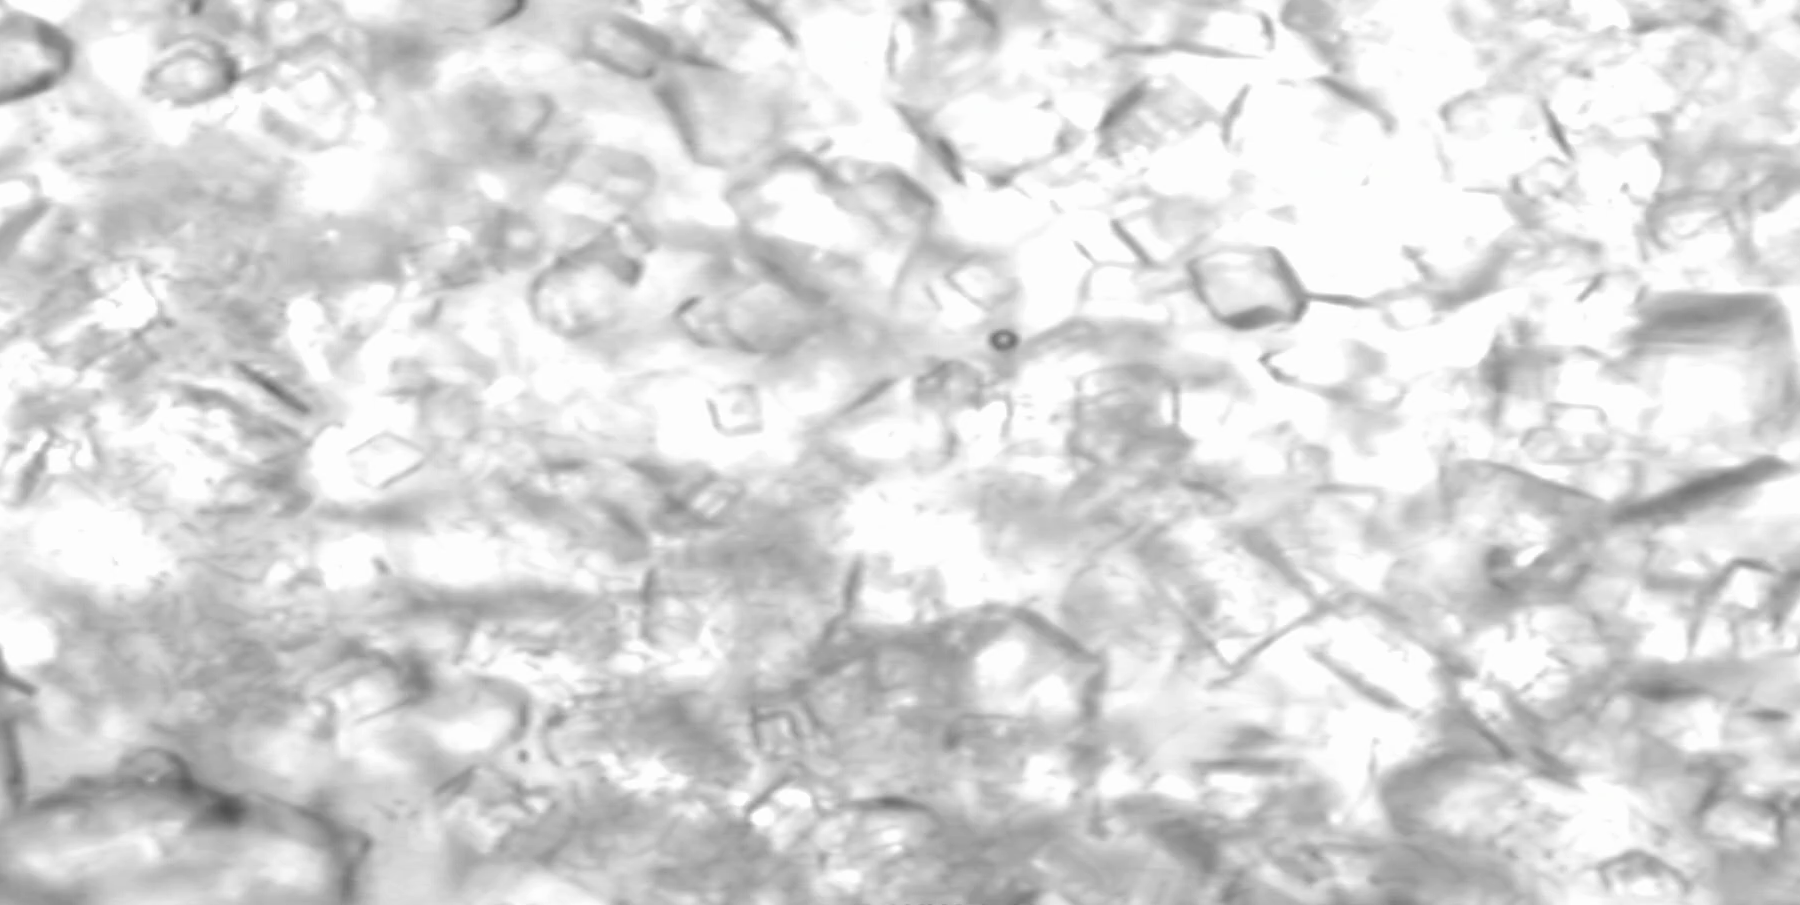
\includegraphics[width=\linewidth]{00_first_frame_cropped}
\caption{\textbf{What does the pipeline's input look like after frame conditioning?} Same frame after the two-step
crop removes both the DVR overlay and the analogue-aspect black bars ($1800 \times 905$~px $\approx 78$\,\% of the
raw frame area). The field is filled with sucrose crystals at varying defocus, with one crystal in focus near the
centre and progressively defocused crystals toward the periphery --- \emph{and no contamination sources left}.
Compare \secref{sec:empirical} for the quantitative impact of the crop on the measured Laplacian-variance $\alpha$
exponent.}\label{fig:frames-cropped}
\end{subfigure}
\caption{Raw and cropped first frame of the case-study video.}\label{fig:frames}
\end{figure}

% Section 3. Grounded rewrite 2026-11-03 (branch docs/cep-grounded-draft). Scale numbers: python -m optics.scale_chain
% (docs/optics/scale_chain.md); other numbers: scripts/rerun_paper_numbers.py --no-video (docs/optics/rerun_results.md).
% Claim changes: papers/cep/CLAIM_CHANGES.md.
\section{Geometric optics through the sight glass \emph{(RQ1)}}\label{sec:optics}

\subsection{Thin-lens scale model}\label{sec:thinlens}

Under the Gaussian thin-lens approximation \citep[\S\,5.2]{Hecht2017}, the object distance $d_o$ and the image
distance $i$ satisfy
\begin{equation}\label{eq:thinlens}
\frac{1}{f} = \frac{1}{d_o} + \frac{1}{i}, \qquad M = \frac{i}{d_o} = \frac{f}{d_o - f},
\end{equation}
with $M$ the transverse magnification. An extension tube of length $e$ sets the image distance at infinity focus
to $f + e$ \citep{PhotonsToPhotos2024}, and the focus helicoid adds its travel $x$, so that
$i = f + e + x = 96$~mm and the focused object distance is $d_\mathrm{focus} = f i / (i - f) = 55.08$~mm, with
$M = 1.743$ (\tabref{tab:inputs}; \code{scripts/rerun_paper_numbers.py}). Once focus is set, $i$ is fixed. A point
at lateral position $X$ and depth $d_o$ is imaged, sharp or blurred, about the chief ray through the lens centre,
at $X i / d_o$ on the sensor. The object-plane extent of one recorded pixel of sensor-plane pitch $p_k$ along axis
$k \in \{x, y\}$ is therefore
\begin{equation}\label{eq:pixelsize}
\Delta_k(d_o) = \frac{p_k}{M(d_o)} = p_k \, \frac{d_o}{i},
\end{equation}
linear in $d_o$ (\figref{fig:mmpx}), with the pitches $p_x \neq p_y$ of the signal chain (\secref{sec:chain}). At
the focused plane $\Delta_k = p_k f / (e + x)$, so the scale there depends only on $f$, $e$ and
$x$.

\begin{figure}
\centering
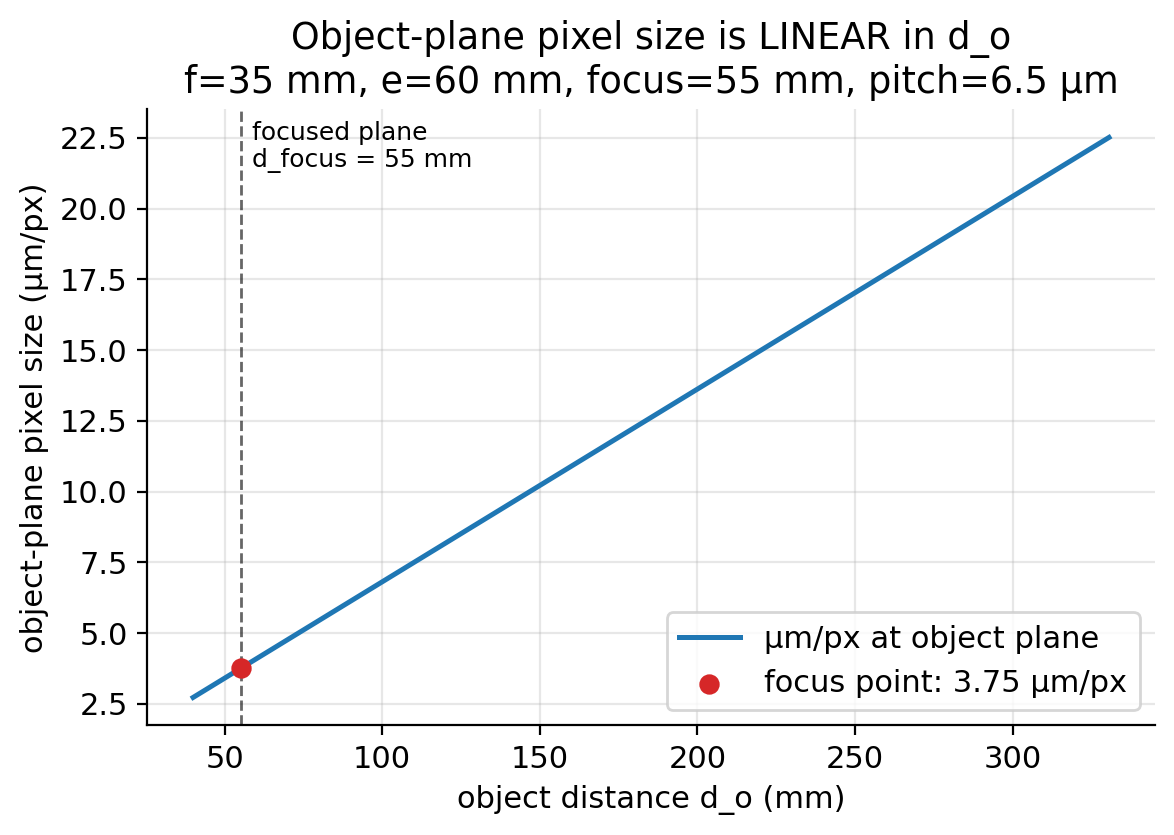
\includegraphics[width=\columnwidth]{01_mm_per_pixel}
\caption{\textbf{How does the metric scale change with depth?} Object-plane extent of one PAL sample, taken as the
geometric mean of its two axes (6.53~\um{} on the sensor), against object distance for $f = 35$~mm, $e = 60$~mm and
$x = 1$~mm. The curve is linear in $d_o$ (Eq.~\ref{eq:pixelsize}); at the focused plane it is 3.75~\umpx. The
per-axis values are given in \tabref{tab:scale}.}\label{fig:mmpx}
\end{figure}

\subsection{Pixel scale at the focused plane and its uncertainty}\label{sec:budget}

\tabref{tab:scale} gives the per-axis scale of both recording types at the focused plane
(\code{python -m optics.scale_chain}; \code{docs/optics/scale_chain.md}). The uncertainty comes from a Monte Carlo
propagation over 200\,000 draws of the inputs of \tabref{tab:inputs}: $e$ uniform within $\pm 5$~mm (the plant's
``$\approx 6$~cm'' read as rounded to the centimetre), $x$ uniform over 0--2~mm, $f$ normal with $\sigma = 2$\,\%
(assumed lens tolerance), the line-to-sample mapping uniform within $\pm 2$\,\% (x only), the camera candidate
(x up to $+0.6$\,\%, y up to $+0.8$\,\%) and the measured 1080p stretch ($\pm 0.1$\,\%). Every entry is an estimate:
it inherits the approximate tube length and the unconfirmed camera model.

\begin{table}
\centering\tabfont
\caption{Object-plane pixel scale at the focused plane, \umpx{} (median and 95\,\% interval of the Monte Carlo
budget; nominal in brackets). Last column: the same if the stated tube length includes a 5~mm CS-to-C ring.
Source: \texttt{python -m optics.scale\_chain}.}\label{tab:scale}
\begin{tabular}{@{}llrrr@{}}
\toprule
Recording & Axis & Median [nominal] & 95\,\% interval & With ring \\
\midrule
PAL $720 \times 576$ & x & 3.932 [3.919] & 3.576--4.347 & 4.283 \\
PAL $720 \times 576$ & y & 3.601 [3.586] & 3.285--3.967 & 3.923 \\
1080p clip & x & 1.469 [1.464] & 1.336--1.624 & 1.600 \\
1080p clip & y & 1.921 [1.913] & 1.752--2.116 & 2.092 \\
\bottomrule
\end{tabular}
\end{table}

The 95\,\% interval is about $\pm 10$\,\% on either axis ($\pm 9.8$\,\% along x, $\pm 9.5$\,\% along y), and the
tube length dominates it: $e \pm 5$~mm alone moves the scale by $-7.6$ to $+8.9$\,\%, against $\pm 2.0$\,\% for the
focal-length tolerance, $\pm 2.0$\,\% for the line mapping, $-1.6$ to $+1.7$\,\% for the focus travel and less than
1\,\% for the camera candidate. Whether a 5~mm CS-to-C ring is counted in the 60~mm is a discrete alternative,
$+8.9$\,\%, kept outside the interval. The glass index, the glass thickness and the air gap do not enter: a
parallel plate moves the focused plane but leaves the magnification at a fixed $i$ unchanged. A caliper reading of
$e$ and a photograph of the mount would remove the two largest terms.

For sizes, the per-axis scale matters. A clip pixel is 1.464~\um{} wide and 1.913~\um{} tall in the slurry, so a
length measured along a row is 12\,\% shorter and one measured down a column 15\,\% longer than with the
geometric-mean pixel of 1.673~\um, which is appropriate only for areas. The geometric mean of the PAL sample is
3.749~\um; a PAL sample, not a clip pixel, is the resolution element of both recordings (\secref{sec:chain}).

\subsection{Sight-glass refractive shift}\label{sec:shift}

A parallel plate of thickness $t$ and index $n_g$ shifts the apparent object distance toward the lens by
$\Delta = t (1 - 1/n_g)$ in the paraxial limit \citep{Hecht2017}. For $t = 20$~mm and the assumed $n_g = 1.47$,
$\Delta = 6.39$~mm, independent of distance; $n_g = 1.52$ would give 6.84~mm (\figref{fig:shift};
\code{scripts/rerun_paper_numbers.py}). The shift moves the focused plane relative to the glass but, as stated
above, not the scale. The exact projection through a flat port is of high polynomial degree (12th degree for two
refractions with distinct indices, \citealp{Agrawal2012}); we use the paraxial form and have not computed the
residual distortion over the field.

\begin{figure}
\centering
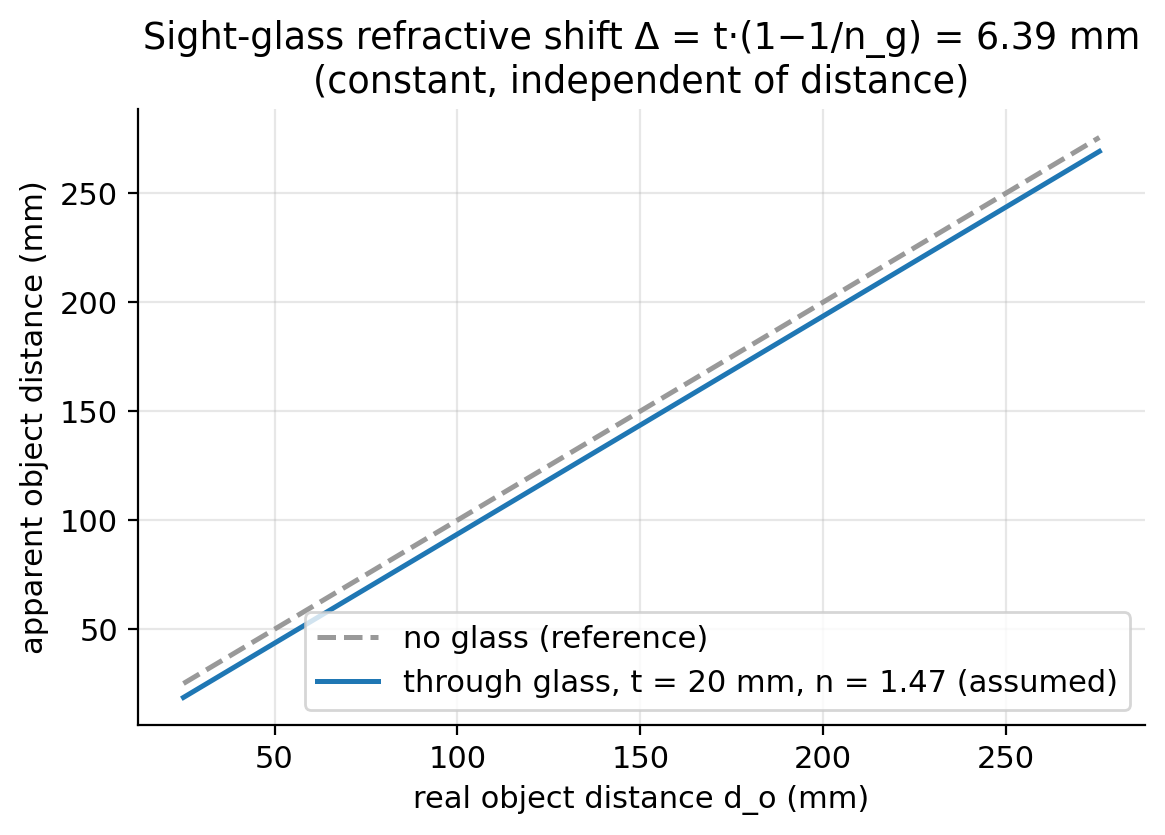
\includegraphics[width=\columnwidth]{05_sight_glass_shift}
\caption{\textbf{How much does the sight glass move the object?} Apparent against real object distance through a
20~mm plate of assumed index $n_g = 1.47$. The paraxial shift is a constant $\Delta = 6.39$~mm; it offsets every
$d_o$ but does not change the slope of \figref{fig:mmpx}.}\label{fig:shift}
\end{figure}

\subsection{Extension-tube sensitivity}\label{sec:tube}

At the focused plane the scale is proportional to $1/(e + x)$ (\secref{sec:thinlens}), so the tube length acts as a
multiplicative factor on every reported size: each $\pm 1$~mm of $e$ or of focus travel moves the scale by
$\mp 1.64$\,\%. \figref{fig:tube} shows the consequence over a standard extension-ring set. A 10~mm tube instead of
60~mm would make the scale 5.55 times coarser, $8.12 \times 10.61$~\umpx{} on a clip pixel.

The tube length cannot be recovered reliably from the image by anchoring a typical crystal size, because that size
changes by more than an order of magnitude within a strike (the microscope medians of \secref{sec:plant} grow from
29 to 483~\um{} in two hours). A wrong tube length would rescale the whole distribution without making it
internally inconsistent. The tube must therefore be measured; in the absence of a caliper reading the plant's
``$\approx 6$~cm'' leaves the $\pm 10$\,\% interval of \tabref{tab:scale}.

\begin{figure}
\centering
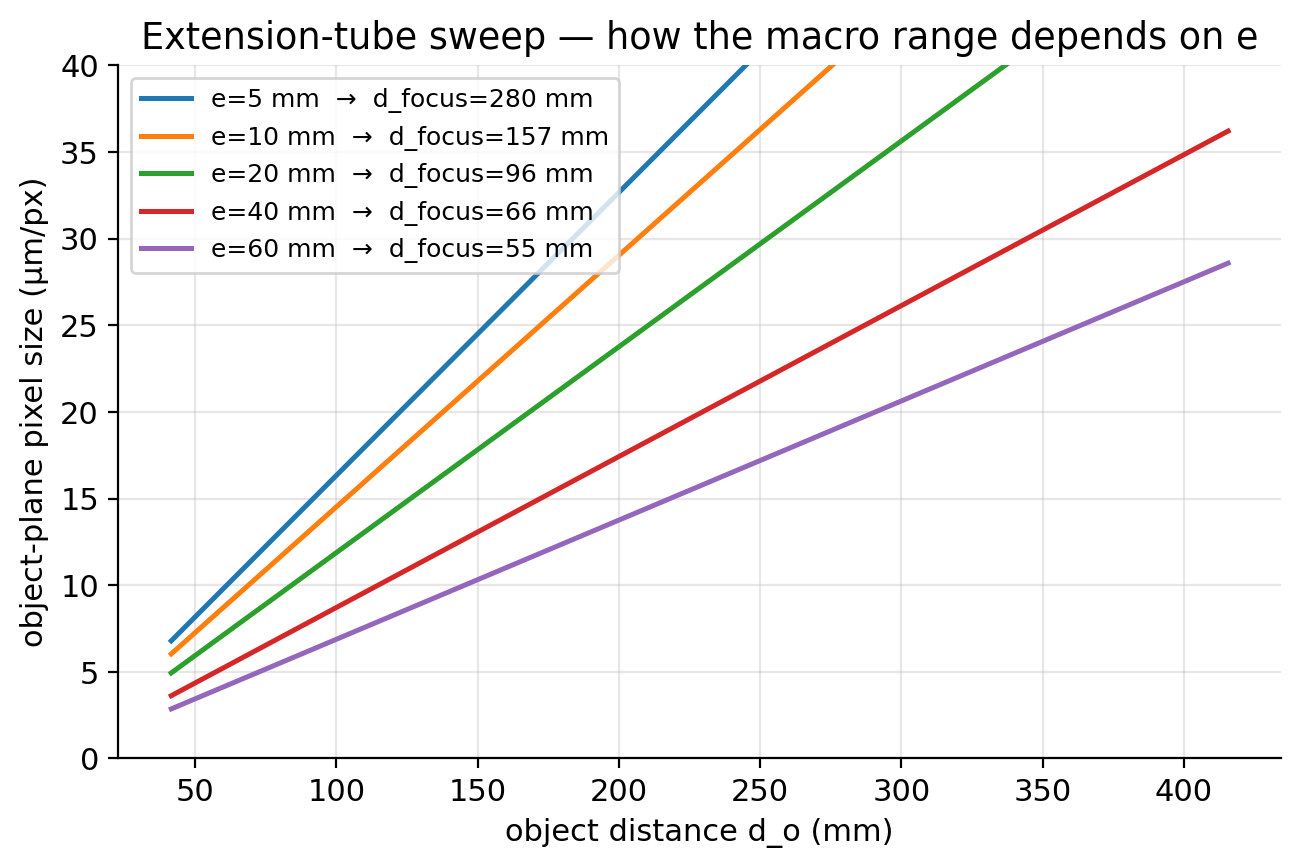
\includegraphics[width=\columnwidth]{06_extension_tube_sweep}
\caption{\textbf{How does the extension tube set the macro range?} Object-plane extent of the geometric-mean PAL
sample against object distance for tube lengths of 5, 10, 20 and 40~mm (an analysis choice) and the installed
${\approx}\,60$~mm. The legend gives the focused distance of each tube; the curves are drawn without the focus
travel, $i = f + e$.}\label{fig:tube}
\end{figure}

\subsection{Where the focal plane sits relative to the glass}\label{sec:slab}

\figref{fig:layout} draws the optical stack to scale. The lens datasheet gives the back focal distance but not the
position of the front principal plane $H$ \citep{FujinonHF35HA1B}, so the focused plane cannot be placed
relative to the glass from the datasheet and the plant geometry alone. The geometry is, however, consistent with a
focal plane at the inner glass face. In that case the real distance from $H$ to the inner face is
$d_\mathrm{focus} + \Delta = 55.08 + 6.39 = 61.47$~mm, and subtracting $t = 20$~mm and $a \approx 20$~mm places $H$
$21.5 \pm 3.4$~mm (1$\sigma$, \code{python -m optics.error_budget}) behind the front element, inside the 30.5~mm lens body (29.5~mm plus the 1~mm focus travel). On the image
side, for a C-mount body, the flange depth of 17.53~mm, the tube and the lens body put the rear principal plane $H'$, which lies
$i = 96$~mm in front of the sensor, 12.0~mm behind the front element (\code{python -m optics.error_budget}). Both
planes then fall inside the lens body. This is a consistency check on the stated geometry, not a measurement of the
focal-plane position. An empty-tank frame in which the scratches of the glass's inner face are sharp would locate
the plane directly.

\begin{figure*}
\centering
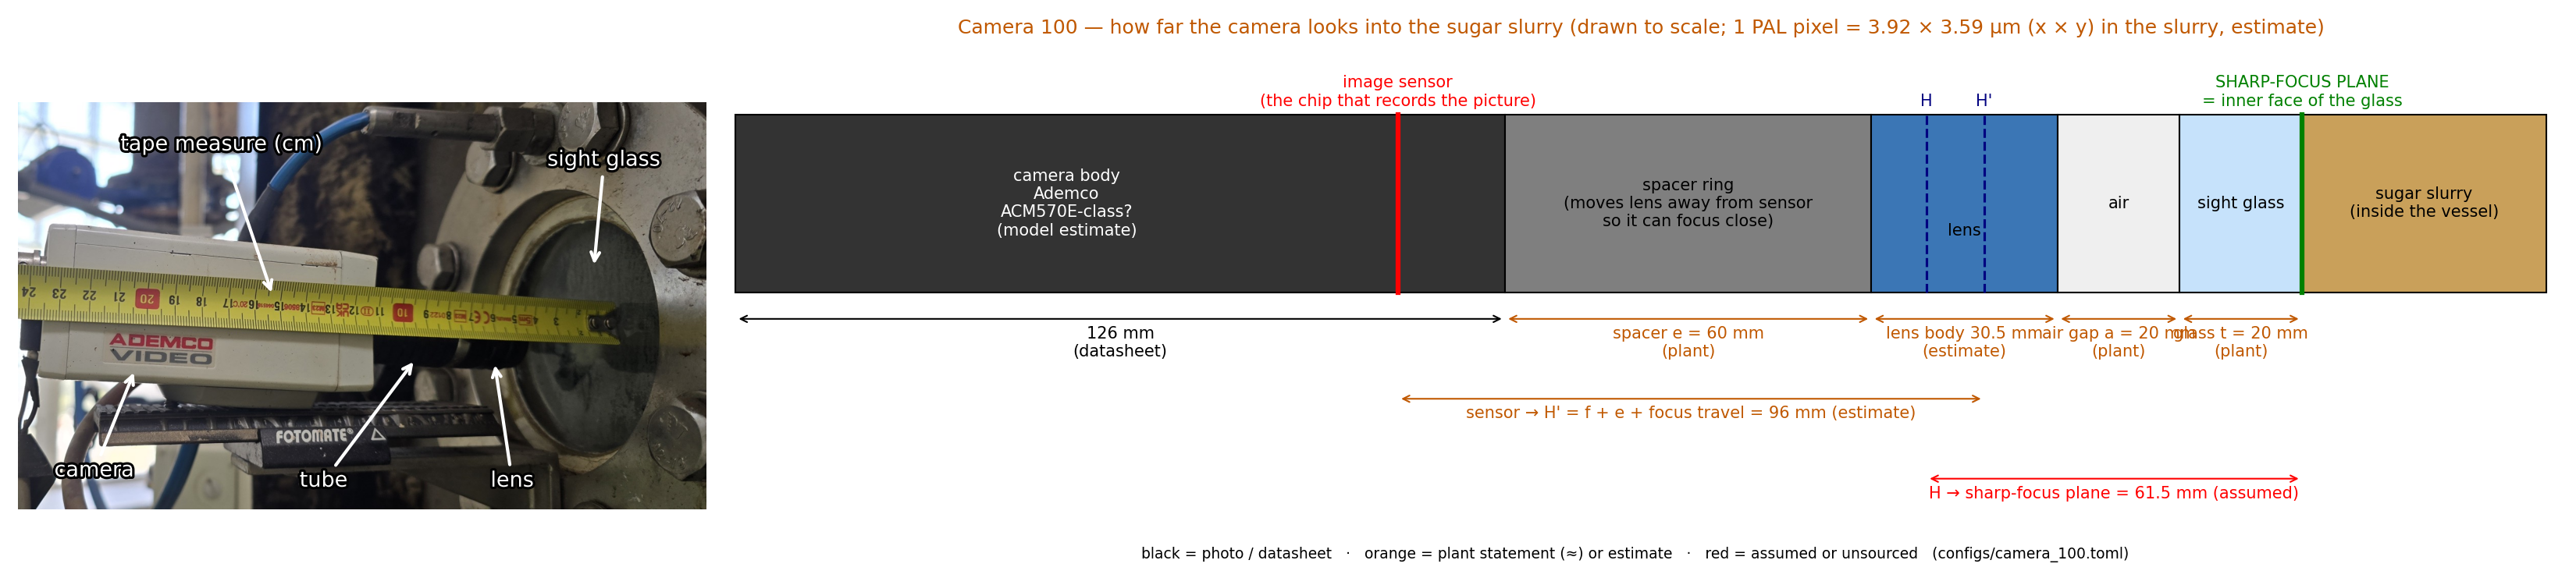
\includegraphics[width=0.85\textwidth]{18_optical_layout}
\caption{\textbf{What does the optical chain from sensor to slurry look like?} Layout drawn to scale from
\texttt{configs/camera\_100.toml} (\texttt{python -m optics.optical\_layout}); the colour of each dimension gives its
source class. Camera body length (40~mm) and lens body (30.5~mm, including the 1~mm focus travel) are estimates;
tube $e$, air gap $a$ and glass $t$ are plant statements; the sensor-to-$H'$ distance $i = f + e + x = 96$~mm is
derived. The placement of the sharp-focus plane at the inner glass face, and hence $H \to$ focus $= 61.5$~mm, is an
assumption (\secref{sec:slab}).}\label{fig:layout}
\end{figure*}

If the focal plane does lie at the inner glass face, the camera samples the slurry layer pressed against the glass,
with an in-focus slice of $\pm 9.4$~\um{} (\secref{sec:dof}). That this layer represents the bulk of the stirred
pan is the homogeneity assumption of \secref{sec:homog}, not a measured fact. The vessel dimensions play no role in
the depth range: the optical slice is far thinner than any vessel dimension.

% Section 4. Grounded rewrite 2026-11-03 (branch docs/cep-grounded-draft). Numbers: scripts/rerun_paper_numbers.py
% (rows 15-18, 21-23, 48-51; docs/optics/rerun_results.md); figures: python -m optics.plots, python -m optics.measure.
% Claim changes: papers/cep/CLAIM_CHANGES.md.
\section{Defocus structure and sharpness profile \emph{(RQ2)}}\label{sec:defocus}

\subsection{Circle of confusion}\label{sec:coc}

For a lens focused at $d_\mathrm{focus}$ with aperture diameter $f / N$, the geometric circle-of-confusion (CoC)
diameter at the sensor for an object at $d_o$ follows from similar triangles and Eq.~\eqref{eq:thinlens}
\citep{Pentland1987}:
\begin{equation}\label{eq:coc}
c(d_o) = K \, \frac{|d_o - d_\mathrm{focus}|}{d_o}, \qquad K = \frac{f^2}{N (d_\mathrm{focus} - f)}.
\end{equation}
The blur is asymmetric in $d_o$: it grows faster on the near side and saturates at $c_\infty = K = 38.12$~mm (F/1.6)
as $d_o \to \infty$. In the reciprocal variable $u = 1/d_o$ it is linear and symmetric about $u_\mathrm{focus}$,
\begin{equation}\label{eq:cocu}
c(u) = K \, d_\mathrm{focus} \, |u - u_\mathrm{focus}|,
\end{equation}
so a blur diameter alone does not tell whether an object lies in front of or behind the focused plane
\citep{SellentFavaro2014}; \secref{sec:sizing} addresses this ambiguity. Close to focus,
$c \approx K |\delta| / d_\mathrm{focus}$ with $\delta = d_o - d_\mathrm{focus}$.

\begin{figure*}
\centering
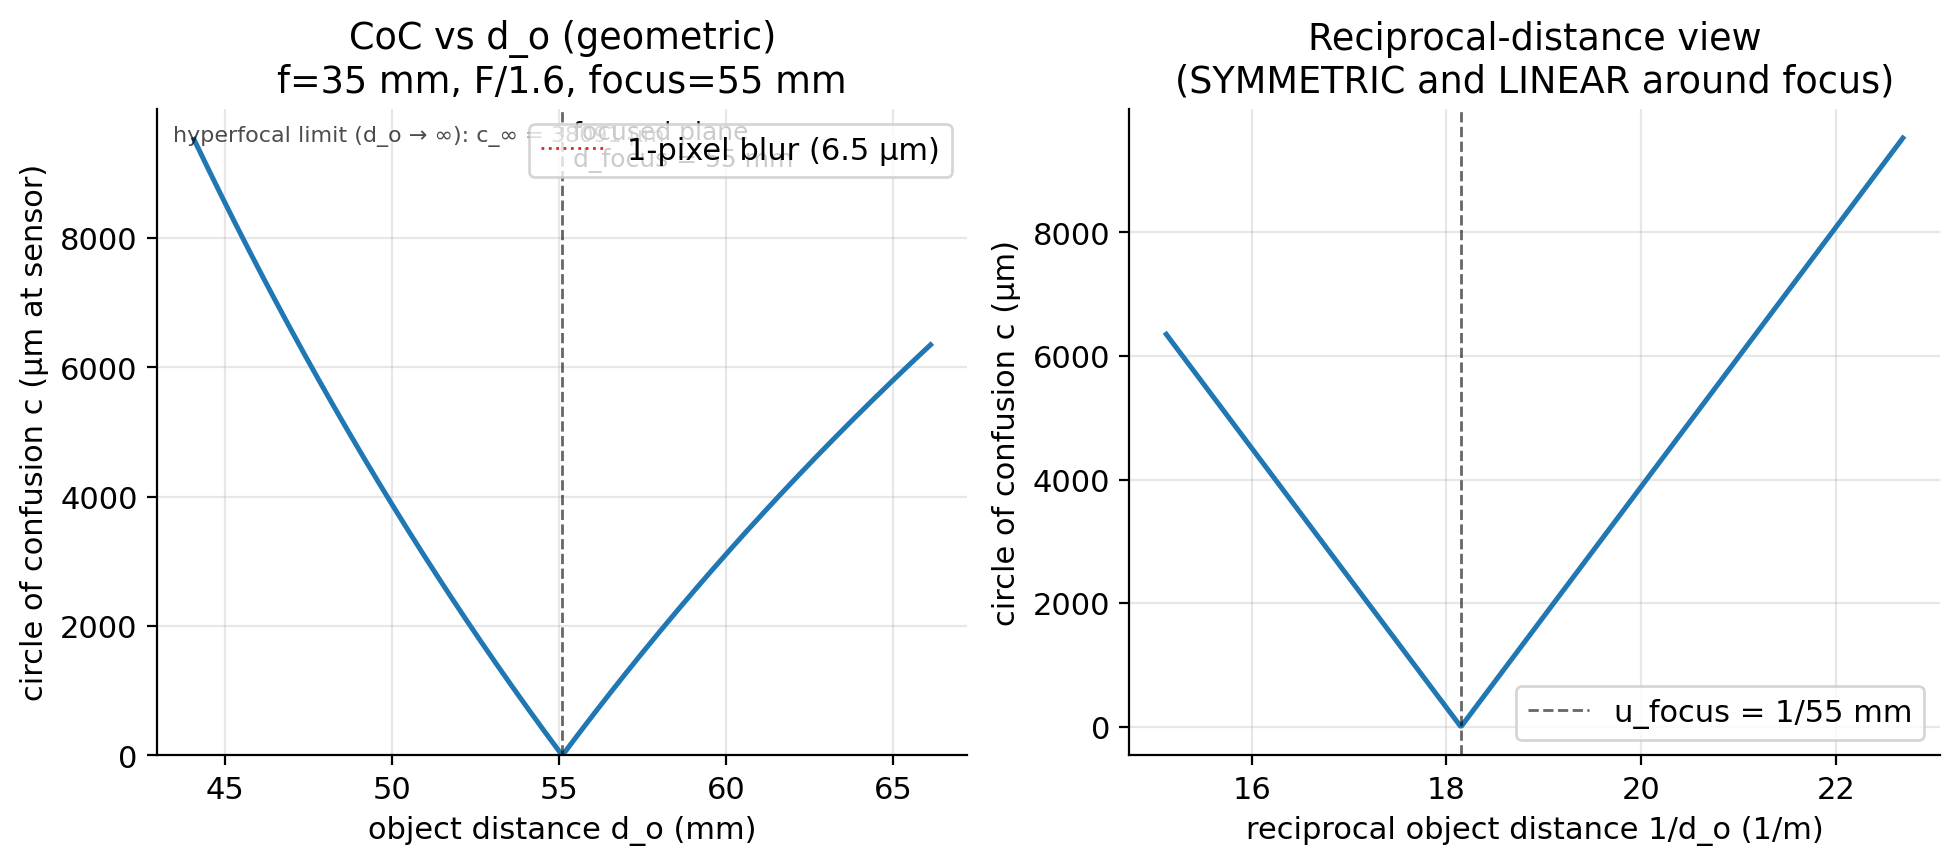
\includegraphics[width=0.85\textwidth]{02_coc_vs_distance}
\caption{\textbf{How does blur grow away from the focused plane?} Geometric CoC at F/1.6 against object distance
(left), asymmetric in $d_o$, and against reciprocal distance $u = 1/d_o$ (right), symmetric and linear about
$u_\mathrm{focus}$. The left CoC axis is logarithmic so that the dotted line of one geometric-mean PAL sample
(6.5~\um{} on the sensor) is visible; the legend gives the limit $c \to K$ for $d_o \to \infty$.}\label{fig:coc}
\end{figure*}

\subsection{Sharpness profile under a Gaussian PSF}\label{sec:psf}

We approximate the defocus point-spread function by a Gaussian whose width is proportional to the blur diameter,
$\sigma = k c$, where the constant $k$ depends on the camera \citep{Pentland1987,SubbaraoSurya1994}. We take
$k = 1/2$; a uniform disk of diameter $c$ would give $c/4$ per axis. The constant sets the width of the sharpness
peak, not its asymptotic exponent. The optical transfer function is then $|H(\nu)|^2 = \exp(-4 \pi^2 \sigma^2 \nu^2)$
at spatial frequency $\nu$. A Laplacian-type focus measure \citep{Pertuz2013} weights the image spectrum by $\nu^4$;
for a one-dimensional integral over a texture with a flat spectrum,
\begin{equation}\label{eq:sharpness}
S(\sigma) \propto \int_0^{\infty} e^{-4 \pi^2 (\sigma^2 + \sigma_0^2) \nu^2} \, \nu^4 \, \mathrm{d}\nu
\propto (\sigma^2 + \sigma_0^2)^{-5/2},
\end{equation}
where the floor $\sigma_0$ combines, in quadrature, half a geometric-mean PAL sample and the diffraction width
$\sigma_\mathrm{diff} \approx 0.42 \lambda N_w$, the Gaussian approximation of the paraxial Airy pattern
$\sigma \approx 0.21 \lambda / \mathrm{NA}$ with the image-side $\mathrm{NA} \approx 1/(2N_w)$
\citep{ZhangZerubia2007}. At macro magnification the working F-number is $N_w = N(1 + M)$, with the pupil
magnification taken as one; at $M = 1.743$ it is $2.74\,N$, and $\lambda = 550$~nm gives a diffraction FWHM at the
sensor of 2.4~\um{} (0.37 PAL samples) at F/1.6 (\code{scripts/rerun_paper_numbers.py}, rows 106--109). The exponent
$5$ is a property of these assumptions, not of the optics alone. The same integral taken in two dimensions over a
texture whose power spectrum falls as $|\nu|^{-\beta}$ gives $(\sigma^2 + \sigma_0^2)^{-(6 - \beta)/2}$. Composed with
Eq.~\eqref{eq:coc}, $S$ is a cusp in object distance: tall and narrow at the focused plane, with tails falling as
$|\delta|^{-5}$ once $\sigma \gg \sigma_0$, and not a Gaussian (\figref{fig:sharpness}).

\begin{figure*}
\centering
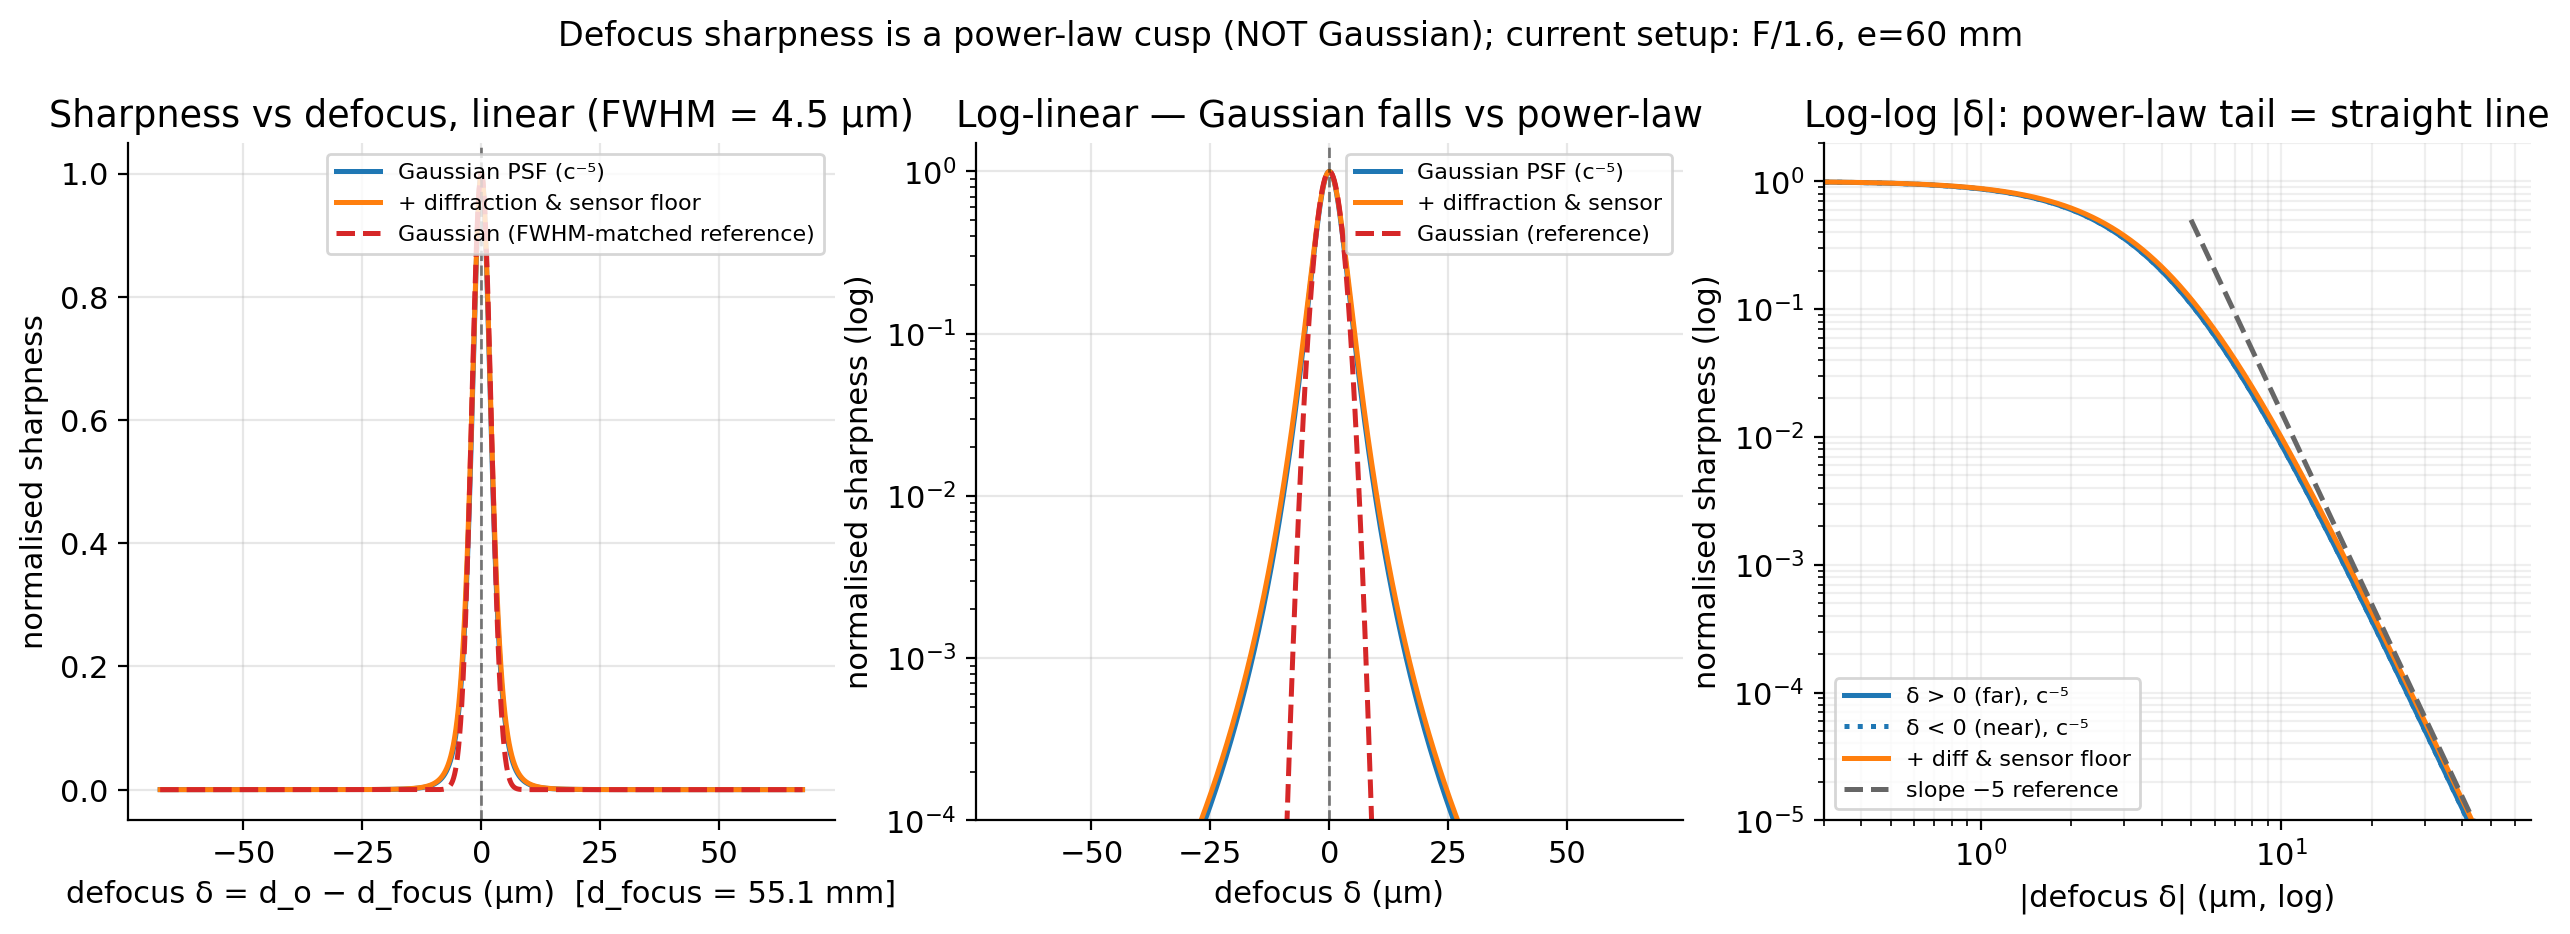
\includegraphics[width=0.82\textwidth]{03_sharpness_vs_distance}
\caption{\textbf{What shape does the model give the sharpness profile?} Modelled sharpness (Eq.~\ref{eq:sharpness})
against defocus $\delta = d_o - d_\mathrm{focus}$ at F/1.6, with the floor set by one PAL sample.
\textbf{Left} (linear): the peak has a full width at half maximum of 10.5~\um{} of object depth; a Gaussian of the
same FWHM is shown dashed. \textbf{Middle} (log $y$): the Gaussian falls off as a parabola, the model has heavy
tails. \textbf{Right} (log--log in $|\delta|$): the model tends to the slope of the $-5$ reference line as $|\delta|$
grows, which restates the model's asymptote and is not a measurement. The diffraction term changes the curve
only near $\delta = 0$.}\label{fig:sharpness}
\end{figure*}

\subsection{Depth of field}\label{sec:dof}

The in-focus slice is the depth range in which the CoC stays below one resolution element. For both recording types
that element is the PAL sample (\secref{sec:chain}), 6.53~\um{} on the sensor as a geometric mean; a 1080p clip
pixel (2.92~\um) is an upscaled fraction of a sample and does not resolve finer detail. \tabref{tab:dof} gives the
slice for both definitions, so that the effect of the choice is visible. With the PAL sample, the in-focus slice at
F/1.6 is $\pm 9.4$~\um. The geometric slice grows in proportion to $N$ (Eq.~\ref{eq:coc}; \figref{fig:dof}), but
diffraction grows with $N_w$: its FWHM reaches one PAL sample at about F/4.4 and is 1.8 samples at F/8 and 3.7
samples (23.9~\um) at F/16. Beyond about F/4 no depth meets the one-sample criterion, so the geometric $\pm 94$~\um{}
at F/16 bounds only the geometric blur and is not an in-focus slice. The iris is the only lever of the installed
hardware on the slice thickness, and diffraction caps it. Depths here are in air-equivalent thin-lens coordinates;
beyond the inner glass face, a paraxial depth in a medium of index $n_s$ is $n_s$ times longer.

The PAL sample as resolution element is an assumption, not a measurement, and it is optimistic. The analogue
bandwidth of camera and recorder is undocumented; even the BT.601 luma passband of 5.75~MHz \citep{ITUBT601}
resolves only about 600 points in the 52~\textmu s active line, against 720 samples; the two
interlaced fields of a moving slurry can halve the vertical resolution; and the H.264 compression of the recordings
removes fine texture. Each would coarsen the element and widen the slice in proportion. A measured edge-spread
function of the analogue chain would settle it \pending{effective resolution of the recorded PAL chain}.

\begin{table}
\centering\tabfont
\caption{In-focus half-slice (geometric CoC $\le$ one resolution element) and sharpness FWHM, in \textmu m of
air-equivalent object depth (\texttt{scripts/rerun\_paper\_numbers.py}, rows 16--18 and 21--23). Element: PAL sample
(6.53~\um) or upscaled clip pixel (2.92~\um). At F/16 the diffraction FWHM alone is 3.7 PAL samples, so that row
bounds the geometric blur only.}\label{tab:dof}
\begin{tabular}{@{}lrr@{}}
\toprule
Quantity & PAL sample & clip pixel \\
\midrule
half-slice, F/1.6 & $\pm 9.4$ & $\pm 4.2$ \\
geometric half-slice, F/16 & $\pm 94$ & $\pm 42$ \\
sharpness FWHM, F/1.6 & 10.5 & 5.5 \\
\bottomrule
\end{tabular}
\end{table}

\begin{figure}
\centering
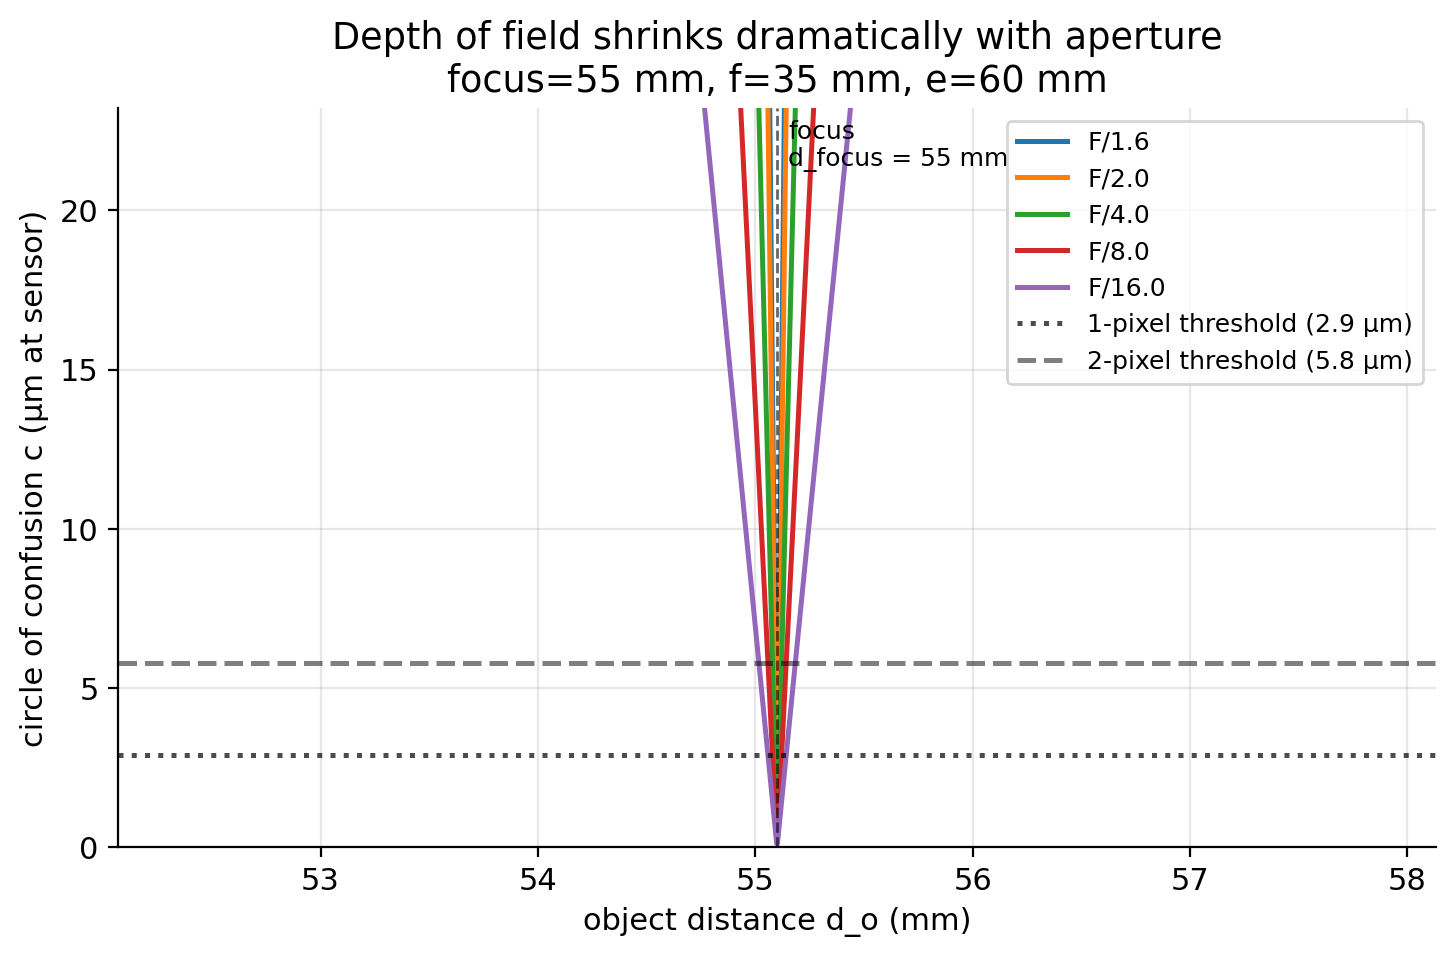
\includegraphics[width=\columnwidth]{04_dof_envelope}
\caption{\textbf{How thick is the in-focus slice at each aperture?} Geometric CoC against object distance for the
engraved iris stops F/1.6, F/2, F/4, F/8 and F/16. Dotted and dashed lines: one and two PAL samples (6.5 and
13.1~\um{} on the sensor). At F/1.6 the CoC stays within one sample over $\pm 9.4$~\um; at F/16 over
$\pm 94$~\um. The curves are geometric; diffraction, not drawn, exceeds one sample beyond about F/4.4
(\secref{sec:dof}).}\label{fig:dof}
\end{figure}

\subsection{Empirical sharpness distribution and frame contamination}\label{sec:empirical}

\code{optics.measure} computes a per-pixel sharpness, $\log(1 + G * (\nabla^2 I)^2)$ with $G$ a $15 \times 15$ Gaussian
kernel, on 120 frames of the case-study clip (every fifth frame), histograms it, and fits a straight line in log--log
coordinates to the density over the band between the 50th and 95th percentiles of its cumulative histogram. The
negative slope $\alpha$ is an empirical descriptor of how fast the density falls past the mode. It is highly
sensitive to the sharp digital and pillarbox edges of \secref{sec:recording} (\tabref{tab:crop}): with no crop
$\alpha = 5.36$, removing the DVR display alone gives 4.57, and removing the pillarbox as well gives 4.88 (fixed
crop) or 4.90 (automatic crop). The two crops that remove both sources agree within 0.4\,\%, whereas the incomplete crops
spread $\alpha$ over 4.57--5.36. Sharp-edged frame contamination must therefore be removed before any sharpness
statistic is interpreted.

\begin{table}
\centering\tabfont
\caption{Fitted slope $\alpha$ of the per-pixel sharpness density for four crops of the case-study clip
(\texttt{scripts/rerun\_paper\_numbers.py}, rows 48--51).}\label{tab:crop}
\begin{tabular}{@{}lr@{}}
\toprule
Crop & $\alpha$ \\
\midrule
none & 5.36 \\
DVR display only (top 55, bottom 120 rows) & 4.57 \\
fixed crop, display and pillarbox ($1800 \times 905$~px) & 4.88 \\
automatic crop, display and pillarbox ($1826 \times 906$~px) & 4.90 \\
\bottomrule
\end{tabular}
\end{table}

We do not read $\alpha$ as a test of the exponent in Eq.~\eqref{eq:sharpness}. That equation describes the sharpness of
an image region as a function of its blur, whereas $\alpha$ describes the distribution over pixels of a smoothed,
log-compressed statistic at unknown and mixed depths. No relation between the two exponents has been derived. Under
the model, a population spread uniformly in depth with $S \propto |\delta|^{-5}$ would give a density of $S$ falling
as $S^{-6/5}$, and a density of $\log S$ falling exponentially rather than as a power law. The closeness of the
cropped $\alpha$ to 5 is therefore not evidence for the model. Directly supported are the crop sensitivity above and
the shape in \figref{fig:measured}: a single mode followed by a shoulder of sharp pixels at a density far below
the peak.

\begin{figure}
\centering
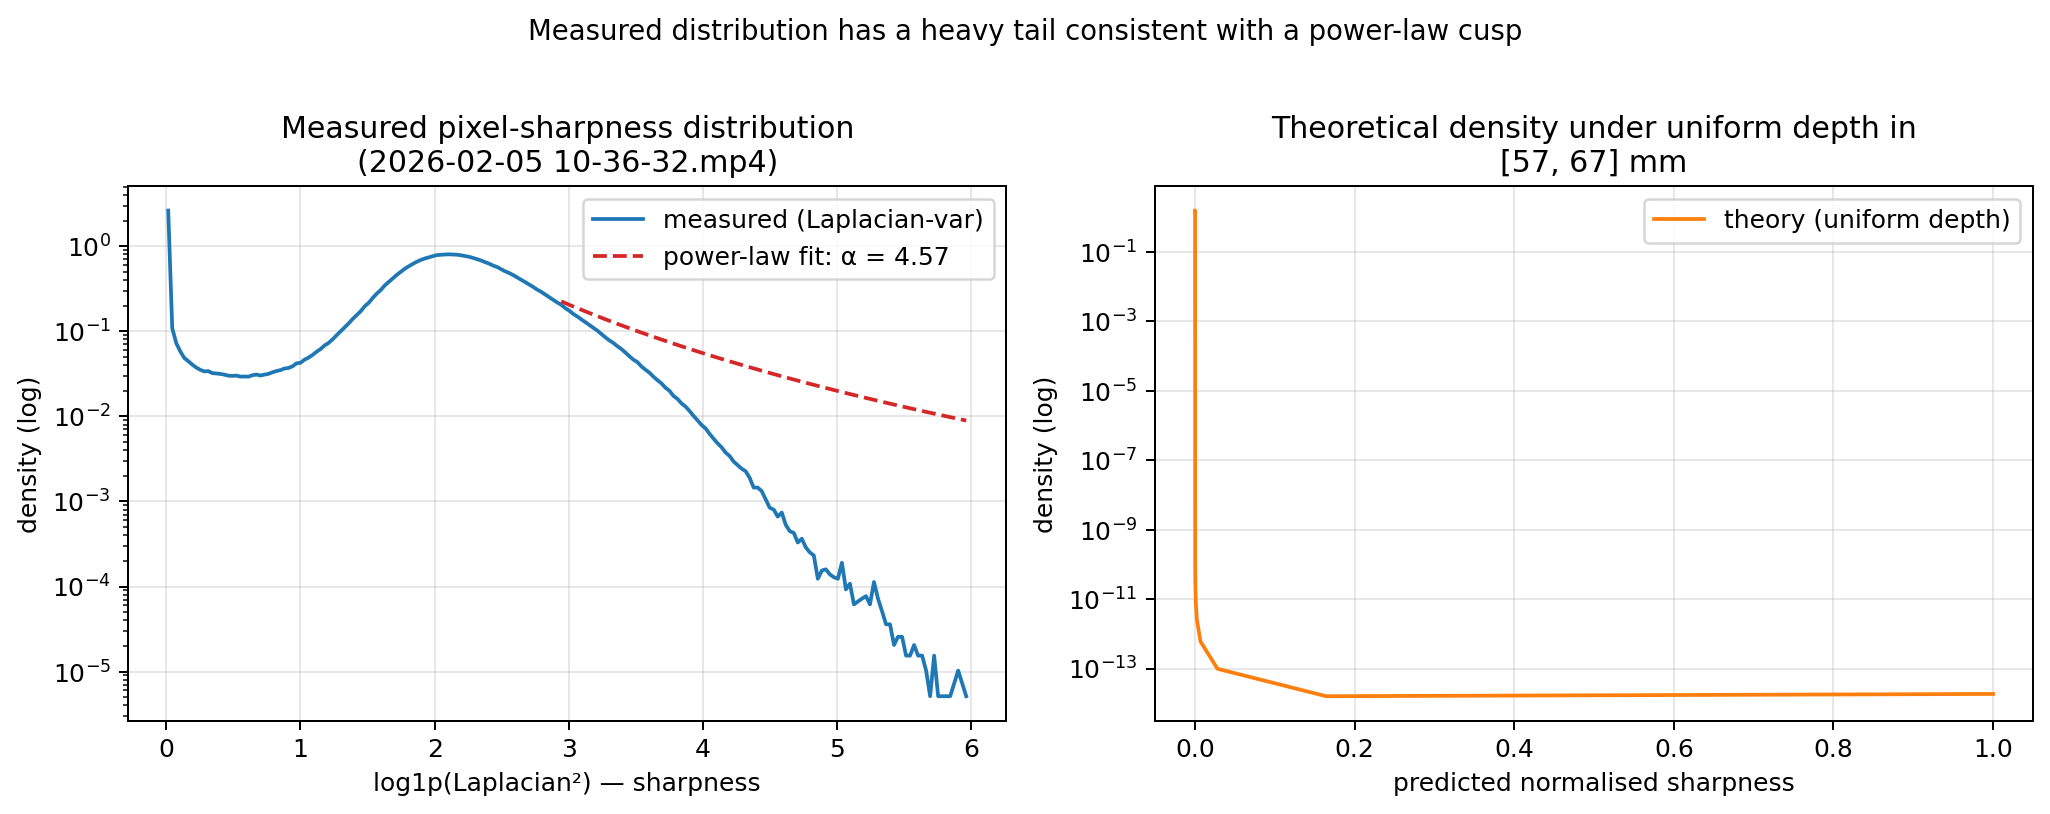
\includegraphics[width=\columnwidth]{08_measured_vs_theory}
\caption{\textbf{What does the measured sharpness distribution look like?} Per-pixel sharpness density of the
case-study clip after the automatic crop (\texttt{optics.measure}). The shaded fit band (50th to 95th percentile of
the cumulative histogram) lies on the decay just right of the mode; the dashed line is the log--log fit over that band,
$\alpha = 4.90$, drawn only where it was fitted. No model density is shown (see text).}\label{fig:measured}
\end{figure}

% Section 5. Rewritten 2026-11-03 (branch docs/cep-grounded-draft) from the code as implemented and the rerun in
% docs/optics/rerun_results.md (scripts/rerun_paper_numbers.py). Claim changes: papers/cep/CLAIM_CHANGES.md.
\providecommand{\pending}[1]{\textbf{[PENDING: #1]}}% defined in main.tex; fallback for standalone builds
\section{Crystal detection as implemented}\label{sec:detection}

This section describes the two classical detectors exactly as the code runs them, the size window they apply and the
depth range they admit. Their output is analysed in \secref{sec:csd}; none of it has yet been compared with
hand-labelled crystals (\secref{sec:validation}).

\subsection{Frame conditioning and sharpness layers}\label{sec:layers}

Each frame of the case-study clip is cropped to the live camera picture. The automatic crop of
\code{optics.video_io.resolve_crop} keeps $1826 \times 906$ of the $1920 \times 1080$ clip pixels (80\,\%); the
single-frame figures use the fixed crop of $1800 \times 905$~px (79\,\%). At the modelled scale of \secref{sec:budget}
($1.464 \times 1.913$~\umpx{} at focus; $\pm\,{\approx}10$\,\% input budget, not validated in the image) the
automatic crop covers
${\approx}\,2.7 \times 1.7$~mm of slurry.

A per-pixel sharpness map is computed as the logarithm of the squared Laplacian smoothed by a $15 \times 15$~px
Gaussian (\code{annotator.sharpness}). A depth score combines the min--max-normalised inverse sharpness (weight 0.7)
with the normalised Farneb\"ack optical-flow magnitude to the previous sampled frame (weight 0.3; zero for a single
frame). The score is quantised uniformly into $L = 3$ layers, and each detector runs once per layer
(\figref{fig:detection} colours detections by layer). The layers order pixels by sharpness and motion; they are not depth measurements, because a
sharpness value maps to two depths (\secref{sec:ambiguity}).

\subsection{Edge and watershed detectors}\label{sec:edge}

Both detectors start from the same Gaussian adaptive threshold (block 11~px, offset 2), which marks the dark crystal
outlines on the bright background.

\emph{Edge detector} (\code{annotator.detection}). The outline map is closed morphologically with an elliptical
kernel of $3 + 4\ell$~px for layer $\ell$; external contours are fitted with minimum-area rotated rectangles, and a
contour is kept if its area lies in the size window (\secref{sec:window}) and its aspect ratio is at most~3.

\emph{Watershed detector} (\code{optics.detect_watershed}). The outline map is opened with a $3 \times 3$ kernel and
its complement is distance-transformed. Seeds are the h-maxima ($h = 2.5$~px) of the distance map that lie at least
6~px from any outline and at least 12~px from each other (\tabref{tab:ws-constants}). A marker-controlled watershed
on the negative distance map, a standard image-segmentation method~\citep{Vincent1991,BeucherMeyer1993}, grows one
basin per seed; each basin is fitted and filtered as above, with the basin pixel count as its area.

\begin{table}
\centering\tabfont
\caption{Seed constants of the watershed detector (CHOICE, module constants of \texttt{optics.detect\_watershed}). The
\textmu m values use the modelled 1080p clip scale of \secref{sec:budget}.}\label{tab:ws-constants}
\begin{tabular}{@{}lr>{\raggedright\arraybackslash}p{0.5\columnwidth}@{}}
\toprule
Constant & Value & Role \\
\midrule
\code{_PEAK_MIN_DISTANCE} & 12~px & minimum seed spacing; $17.6 \times 23.0$~\um{} ($x \times y$) \\
\code{_PEAK_THRESHOLD_ABS} & 6~px & minimum distance of a seed from any outline \\
\code{_H_MAXIMA_PARAM} & 2.5~px & h-maxima height; suppresses plateau peaks \\
\bottomrule
\end{tabular}
\end{table}

A detection's size is the geometric mean $\sqrt{w h}$ of its rectangle sides, converted with the geometric-mean
pixel scale ($1.673$~\umpx{} on the clips). Because a pixel is not square (\secref{sec:chain}), this
area-equivalent size is exact under the anisotropic scale, whereas a chord length in a given direction is not: a
pixel spans 1.464~\um{} along a row and 1.913~\um{} down a column, $-12$\,\% and $+14$\,\% of the geometric mean.

\subsection{Size window from the configuration}\label{sec:window}

The area window is read from \code{configs/camera_100.toml} by \code{optics.config.detection_area_px}. Its lower
bound is $3^2 = 9$~px$^2$ (\code{min_side_px} $= 3$, CHOICE). Its upper bound is the pixel area of a 1~mm square at
the focused plane, $\mathit{max\_size}^2 / (\mu_x \mu_y)$ with the per-axis scales $\mu_x, \mu_y$; the 1~mm
(\code{max_size_um}, CHOICE) rounds up the 0.821~mm largest crystal of the first microscope reading
(\secref{sec:expected}). On the 1080p clips the window is $[9,\ 356\,474]$~px$^2$, an area-equivalent 5--1000~\um;
on the PAL recording it is $[9,\ 71\,020]$~px$^2$. Three clip pixels are $4.4 \times 5.7$~\um{} but only
${\approx}\,1.1$ PAL samples, because the clips are upscaled PAL pictures; on PAL, three samples are
$11.8 \times 10.8$~\um.

The earlier fixed window $[80,\ 8000]$~px$^2$ corresponds on the clips to an area-equivalent 15--150~\um{}
(13--131~\um{} along a row, 17--171~\um{} down a column). It is reported below only to show how the detector output
depends on the window.

\begin{figure}
\centering
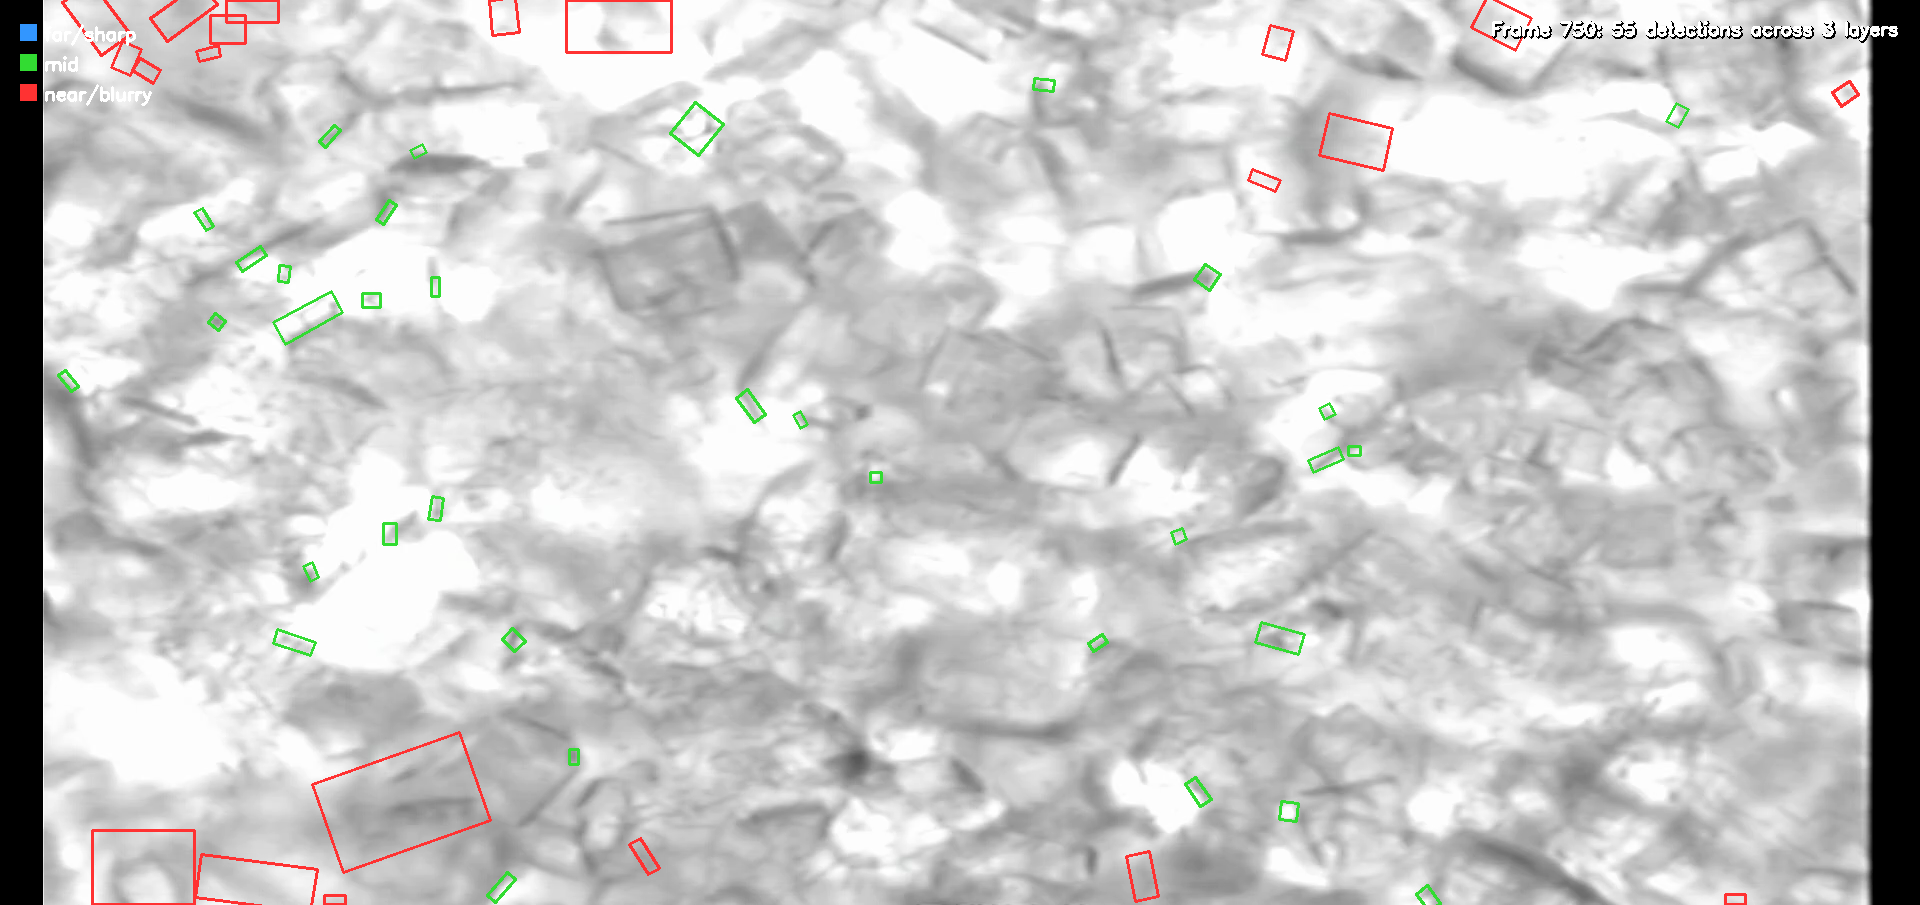
\includegraphics[width=\columnwidth]{11_detection_overlay}
\caption{Edge-detector output on frame 750 with the configured window (\texttt{optics.qualitative}): 840 rotated
rectangles, coloured by sharpness layer (the legend names are the code's layer names, not depth assignments). By
visual reading, not checked against labels, many of the largest rectangles enclose blurred regions rather than single
crystal outlines. The earlier $[80, 8000]$~px$^2$
window gives 292 detections on the same frame.}\label{fig:detection}
\end{figure}

\subsection{Depth range admitted by the detectors}\label{sec:selectivity}

Both detectors need dark outlines a few pixels wide, so they admit only crystals near the focused plane. The
resolution element of the recording is the PAL sample ($6.83 \times 6.25$~\um{} at the sensor, geometric mean
6.53~\um; \secref{sec:chain}), not the upscaled clip pixel. If a detector loses an outline once the circle of
confusion exceeds five resolution elements (an assumption, not a measured threshold), the F/1.6 lens admits
$\delta = \pm 47$~\um{} around focus (\secref{sec:coc}). Over that range the near/far apparent-size ratio of
\eqref{eq:ratio} departs from one by only 0.17\,\%, whereas a 5\,\% difference requires $\delta \approx 1.3$~mm
(\figref{fig:discrim}). Counting in clip pixels instead gives $\pm 21$~\um{} and 0.08\,\%. The size signal that
\secref{sec:sizing} relies on is therefore negligible for any detection these detectors can make at F/1.6.

\begin{figure}
\centering
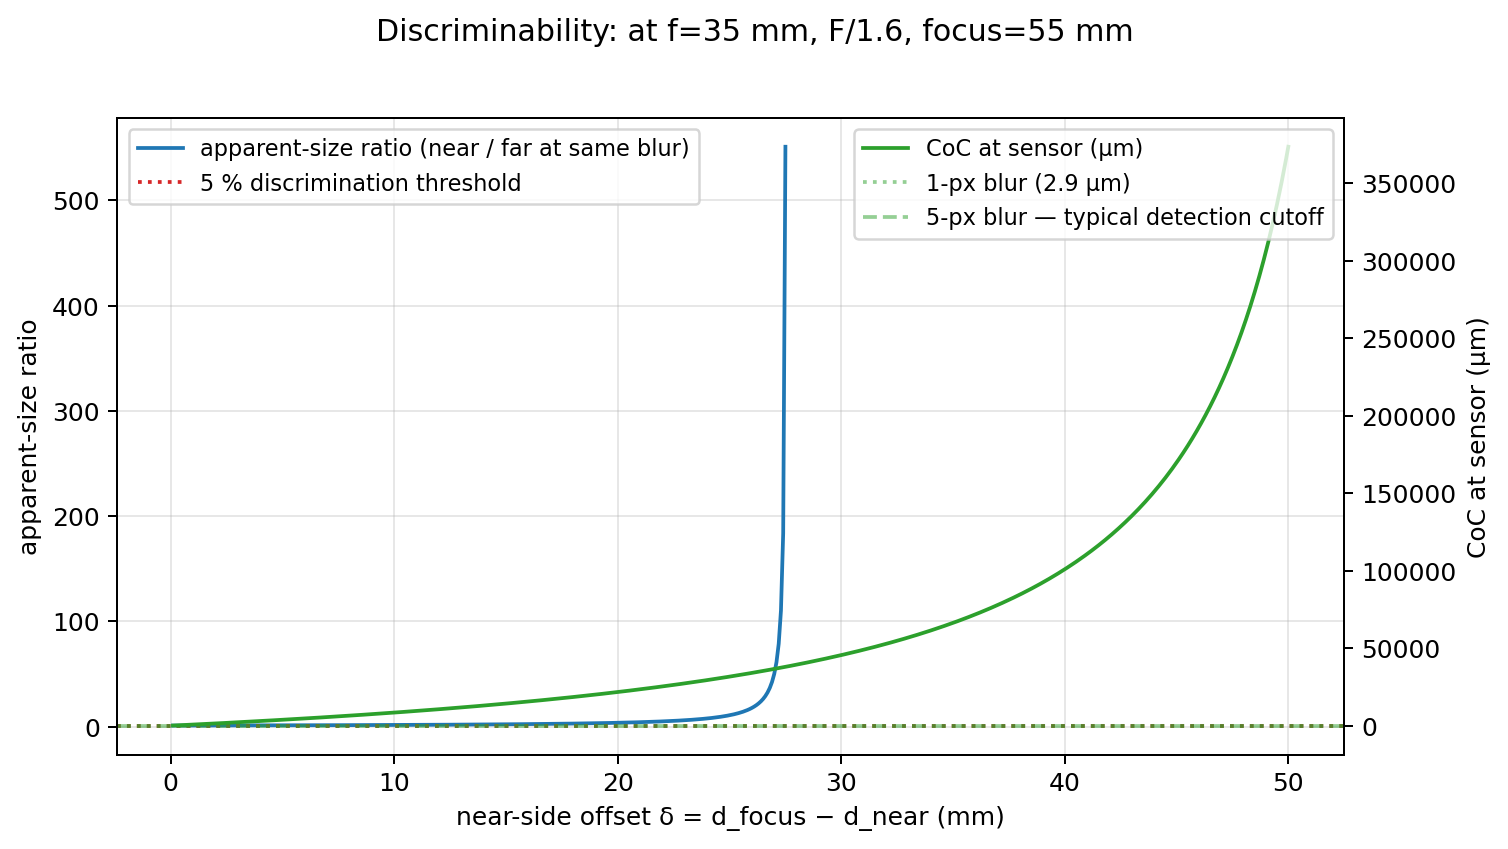
\includegraphics[width=\columnwidth]{10_discriminability}
\caption{Near/far apparent-size difference $d_\mathrm{far}/d_\mathrm{near} - 1$ against the near-side offset
$\delta$ at F/1.6, log axes (\texttt{optics.disambiguate.fig\_discriminability}); the top axis gives the sensor CoC
in PAL samples (6.53~\um). Solid line: in-focus half-slice, 9.4~\um{} (CoC = 1 sample). Dashed: the assumed
five-sample detection cutoff, 47~\um, where the difference is 0.17\,\%. Dotted: 5\,\%, reached at
$\delta \approx 1.3$~mm.}\label{fig:discrim}
\end{figure}

% Section 6. Rewritten 2026-11-03 (branch docs/cep-grounded-draft) from src/optics/disambiguate.py and the rerun in
% docs/optics/rerun_results.md (scripts/rerun_paper_numbers.py). Claim changes: papers/cep/CLAIM_CHANGES.md.
\section{Front/back disambiguation with a single-component size prior}\label{sec:sizing}

\subsection{The front/back ambiguity and the size signal}\label{sec:ambiguity}

Circular-aperture defocus is symmetric in reciprocal object distance (\secref{sec:coc}): two depths with
$1/d_\mathrm{near} + 1/d_\mathrm{far} = 2/d_\mathrm{focus}$ produce the same blur, so a single image does not tell
whether a blurred object lies in front of or behind the focal plane~\citep{SellentFavaro2014}. The apparent size of a
crystal of physical width $w$, however, is monotone in $d_o$. With the pixel scale proportional to object distance,
$\Delta x(d_o) = \Delta x(d_\mathrm{focus})\, d_o / d_\mathrm{focus}$ (\secref{sec:thinlens}),
\begin{equation}\label{eq:spx}
s_\mathrm{px}(d_o) = \frac{w}{\Delta x(d_o)}, \qquad
\frac{s_\mathrm{px}(d_\mathrm{near})}{s_\mathrm{px}(d_\mathrm{far})} = \frac{d_\mathrm{far}}{d_\mathrm{near}},
\end{equation}
\begin{equation}\label{eq:ratio}
\frac{d_\mathrm{far}}{d_\mathrm{near}} - 1 \approx \frac{2\delta}{d_\mathrm{focus}} \quad
(\delta = d_\mathrm{focus} - d_\mathrm{near} \ll d_\mathrm{focus}).
\end{equation}
Equal blur with unequal apparent size is the signal a size prior can exploit. Its strength is set by $\delta$, that
is, by how far from focus the detector still finds crystals (\secref{sec:selectivity}).

\subsection{Homogeneous slurry and a single-component prior}\label{sec:homog}

We assume a homogeneous slurry: the physical size distribution $P_w$ is the same at every depth in the observed slab.
Near and far are then two hypotheses about each detection, not two populations, and the aggregated sizes form one
distribution rather than a mixture. The prior $P_w$ is estimated once from the sharpest detections, converted at
$\Delta x(d_\mathrm{focus})$. A multimodal result would indicate that the assumption fails, for example by
size-dependent settling near the glass.

\subsection{Implementation}\label{sec:impl}

The step is implemented in \code{optics.disambiguate.disambiguate}:
\begin{enumerate}
\item Each detection receives the mean of the smoothed squared Laplacian inside its rectangle, normalised by the
99.5th percentile of all detections, $S \in [0, 1]$.
\item Detections with $S$ at or above the 85th percentile form the focal subset. Their sizes at
$\Delta x(d_\mathrm{focus})$ give $P_w$ as a 60-bin histogram from 0 to 1.5 times its 99th percentile.
\item For every other detection, the Gaussian-PSF sharpness model of \secref{sec:psf} is inverted for the circle of
confusion, $c = 2\sqrt{\sigma_\mathrm{floor}^2 (S^{-2/5} - 1)}$, with $\sigma_\mathrm{floor}$ half a clip pixel, and
$c(d_o) = K\,|d_o - d_\mathrm{focus}|/d_o$ is solved for $d_\mathrm{near}$ and $d_\mathrm{far}$.
\item The implied sizes $w_\mathrm{near}$ and $w_\mathrm{far}$ are looked up in $P_w$, and
$p_\mathrm{near} = P_w(w_\mathrm{near}) / [P_w(w_\mathrm{near}) + P_w(w_\mathrm{far})]$. The detection is labelled
near if $p_\mathrm{near} > 0.5$ and far otherwise, and keeps the size of its label.
\end{enumerate}

\subsection{Result: the prior cannot separate near from far at F/1.6}\label{sec:disamb-result}

On the 60 sampled frames of the case-study clip (watershed detector, configured window), the assigned depths lie
3.1~\um{} (median) and 5.6~\um{} (99th percentile) from $d_\mathrm{focus}$ (\figref{fig:disamb}, middle). By
\eqref{eq:ratio} the two hypotheses then differ in implied size by at most ${\approx}\,2 \times 10^{-4}$, far below
the width of a prior bin, so both look up nearly the same prior density. Accordingly, 99.7\,\% of the off-focus
detections have $p_\mathrm{near}$ within $0.500 \pm 0.002$; the share is 99.6--99.9\,\% for both detectors under
either size window (\tabref{tab:ws-compare}).

The reported near/far splits (76/24 here; 70/30 to 80/20 in the other runs) are therefore produced by the
tie-break rule $p_\mathrm{near} > 0.5$, not by evidence. Because $w_\mathrm{near} < w_\mathrm{far}$, the near label
wins wherever $P_w$ decreases with size, that is, above the prior mode, and the far label wins below it. This
explains why the near and far subsets in \figref{fig:csd} (right) occupy different size ranges. The step does not
change the sizes either: the mean depth correction is 0.005\,\% of the median size. At F/1.6, near/far
disambiguation by a size prior is uninformative, and we do not interpret the splits. The size signal of
\eqref{eq:ratio} becomes usable only if detections are admitted at $\delta$ of order a millimetre
(\figref{fig:discrim}), which needs a smaller aperture or a blur-tolerant detector (\secref{sec:recs}).

\begin{figure*}
\centering
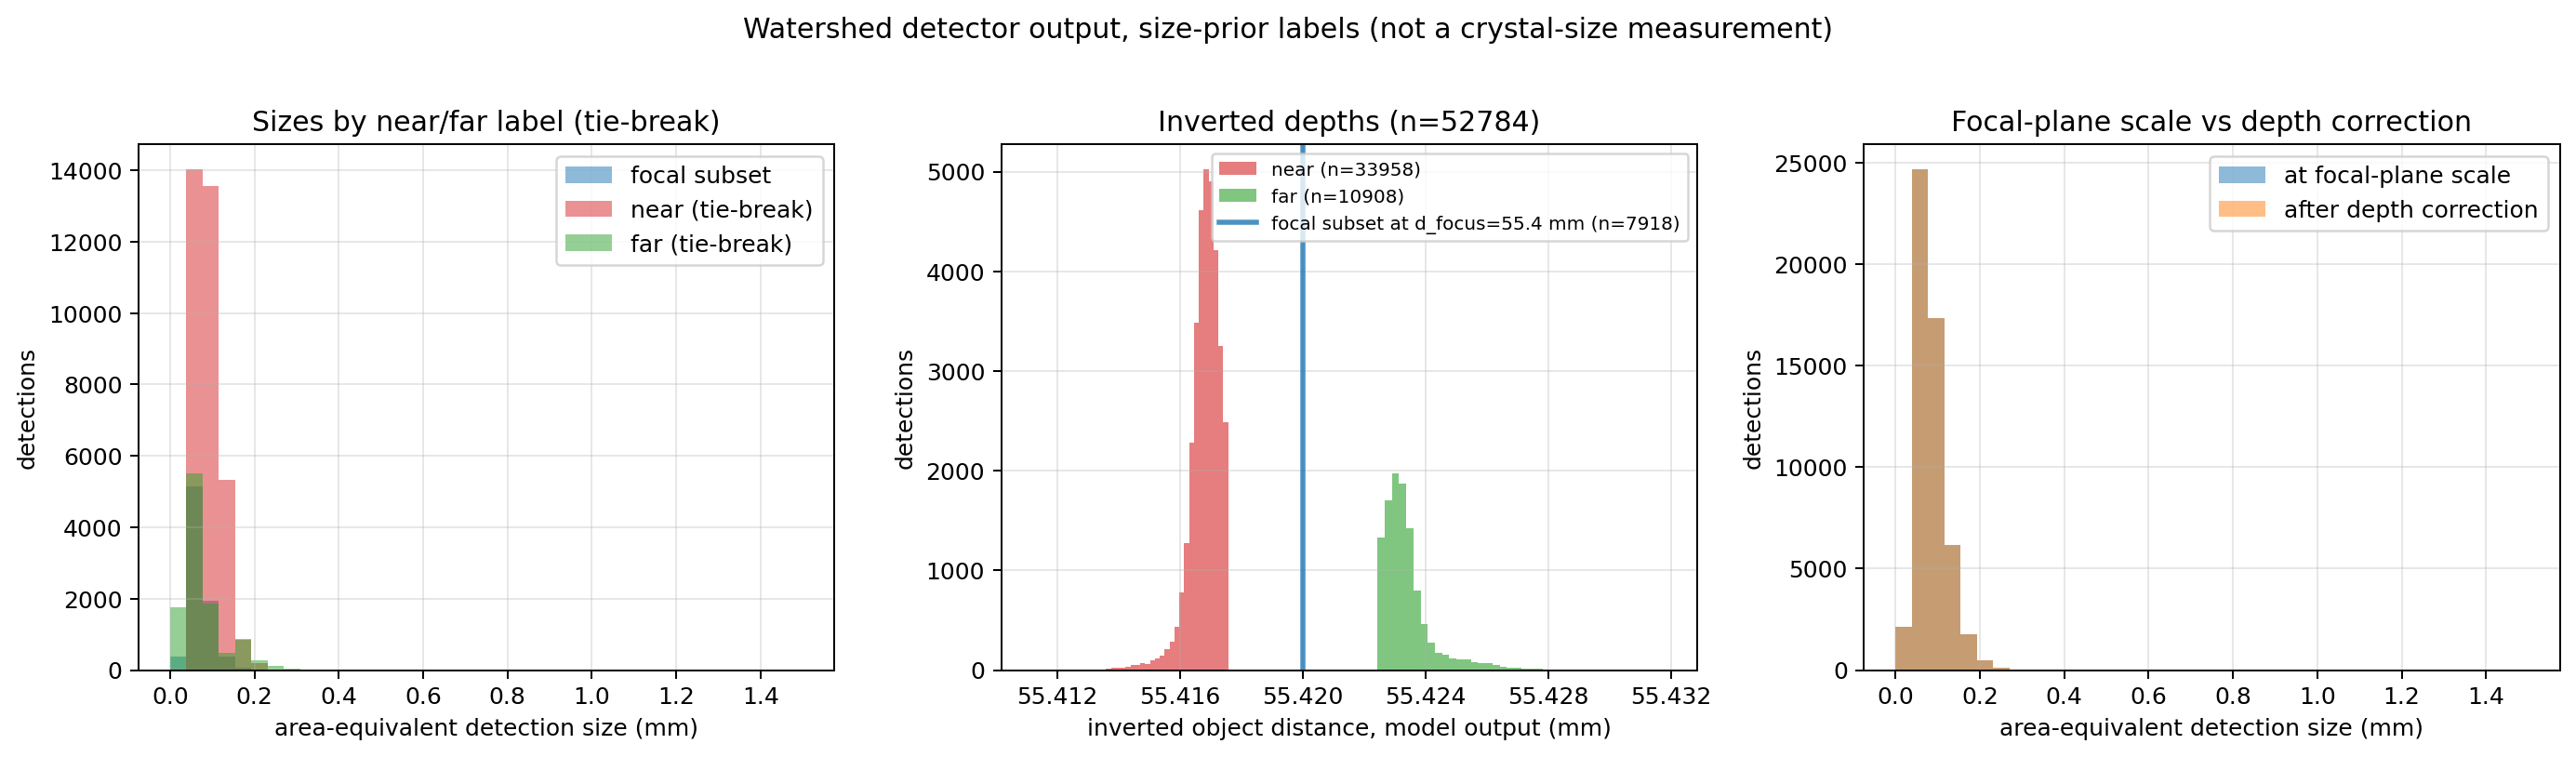
\includegraphics[width=\textwidth]{09_disambiguation}
\caption{Disambiguation output for the case-study clip (\texttt{optics.disambiguate}; watershed detector, configured
window, 52\,784 detections). Left: sizes by label. Middle: assigned depths; the near (33\,957) and far (10\,909)
clusters sit at 55.097 and 55.103~mm, a few micrometres either side of $d_\mathrm{focus} = 55.1$~mm, and 7\,918
detections form the focal subset. Right: sizes at $\Delta x(d_\mathrm{focus})$ and after depth correction; the two
histograms coincide. The near/far labels are tie-break outcomes (\secref{sec:disamb-result}).}\label{fig:disamb}
\end{figure*}

\subsection{Scale overlay at three assumed depths}\label{sec:overlay}

\figref{fig:overlays} draws a 0.1~mm grid and a 1~mm ruler on frame 750 at three assumed object distances. The clip
rows are resampled by 1.306 so that one displayed pixel is the same length on both axes and the grid is true in $x$
and $y$ (\code{scripts/rerun_paper_numbers.py --fig07}). Over $\pm 0.2$~mm the scale changes by $\pm 0.36$\,\%; the
window is 21 times the F/1.6 in-focus half-slice of $\pm 9.4$~\um{} (one PAL sample, \secref{sec:dof}). A single
scale at the focused plane is therefore adequate at this aperture. The sharpness map in the right panels is computed
from the image alone and is identical in all three panels; it shows which pixels carry sharp outlines, not their
depth.

\begin{figure*}
\centering
\begin{subfigure}{\textwidth}
\centering
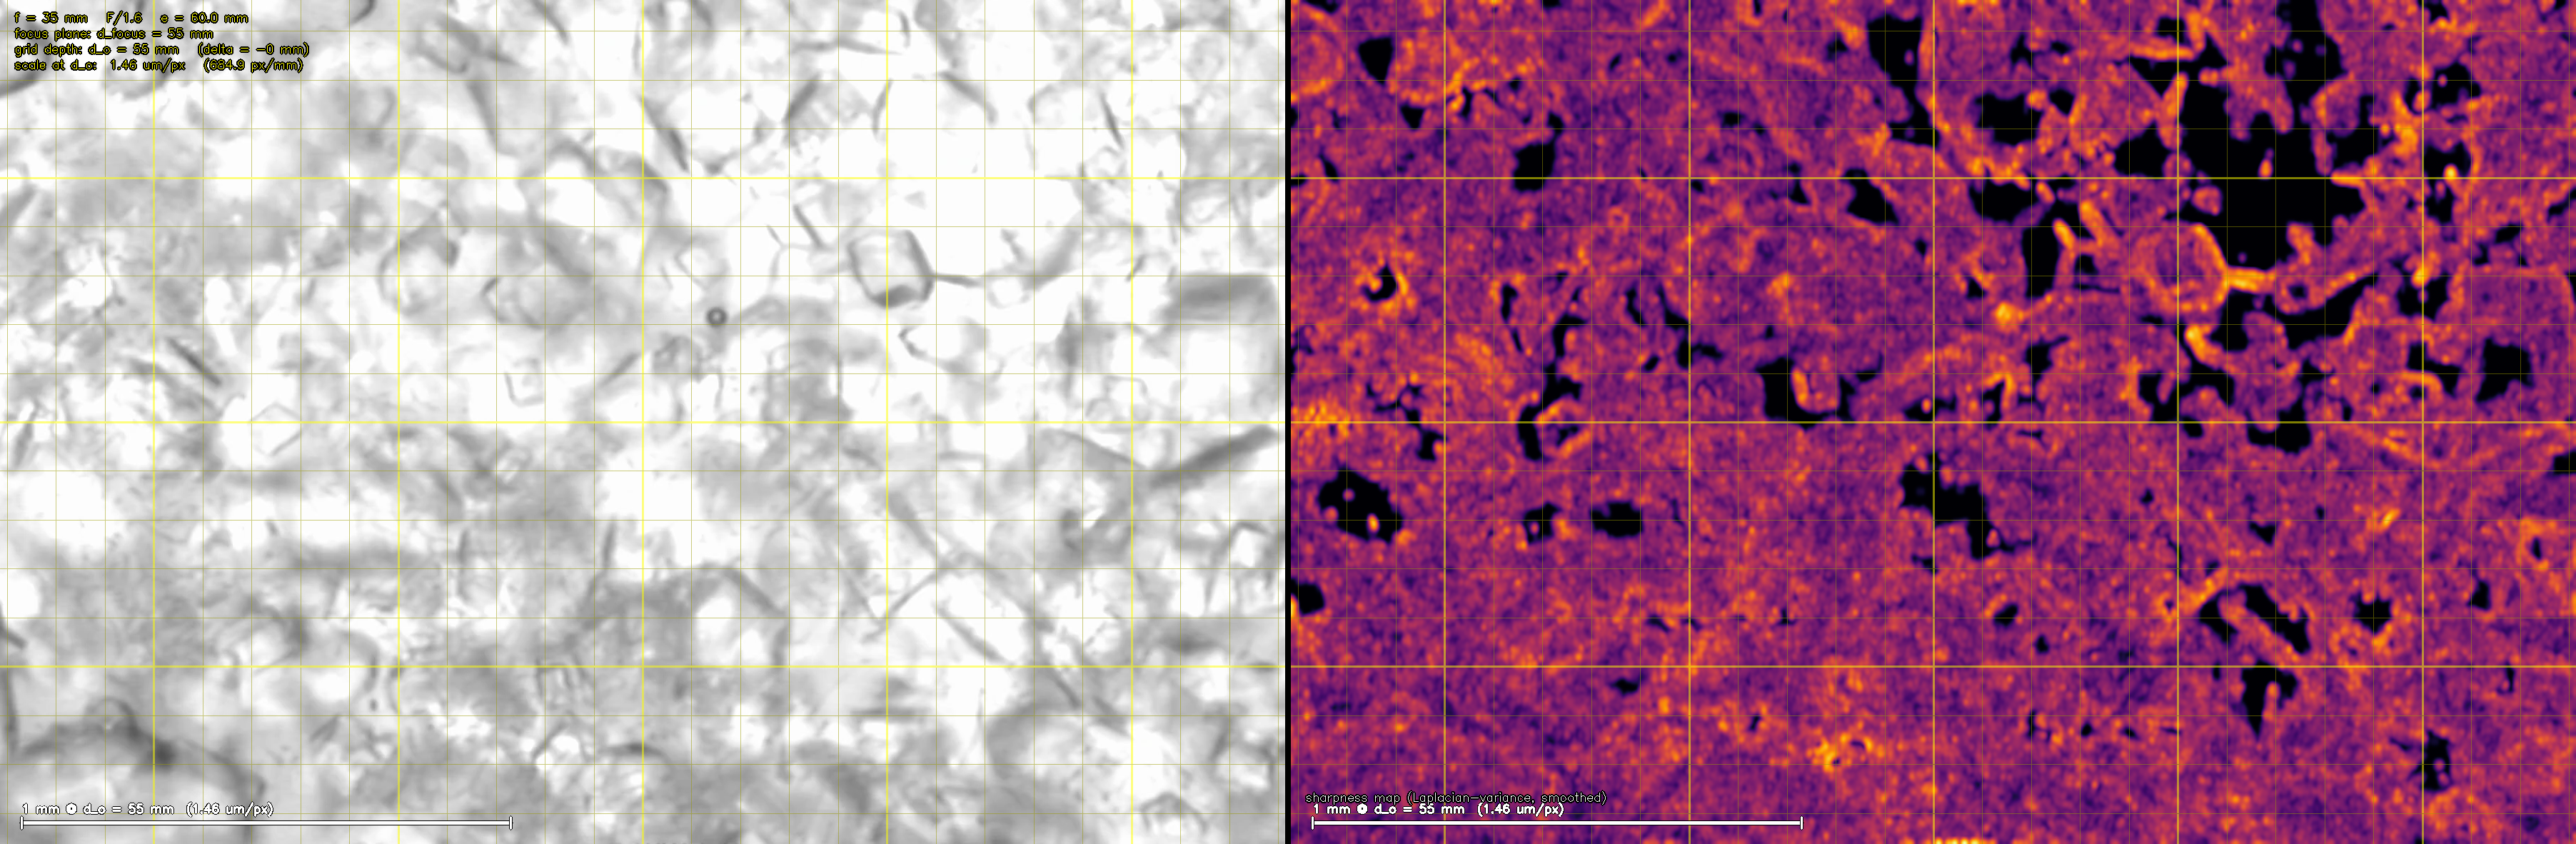
\includegraphics[width=0.8\textwidth]{07_overlay_near}
\caption{$d_o = 54.9$~mm: $1.460 \times 1.907$~\umpx{} ($x \times y$)}\label{fig:overlay-near}
\end{subfigure}

\medskip
\begin{subfigure}{\textwidth}
\centering
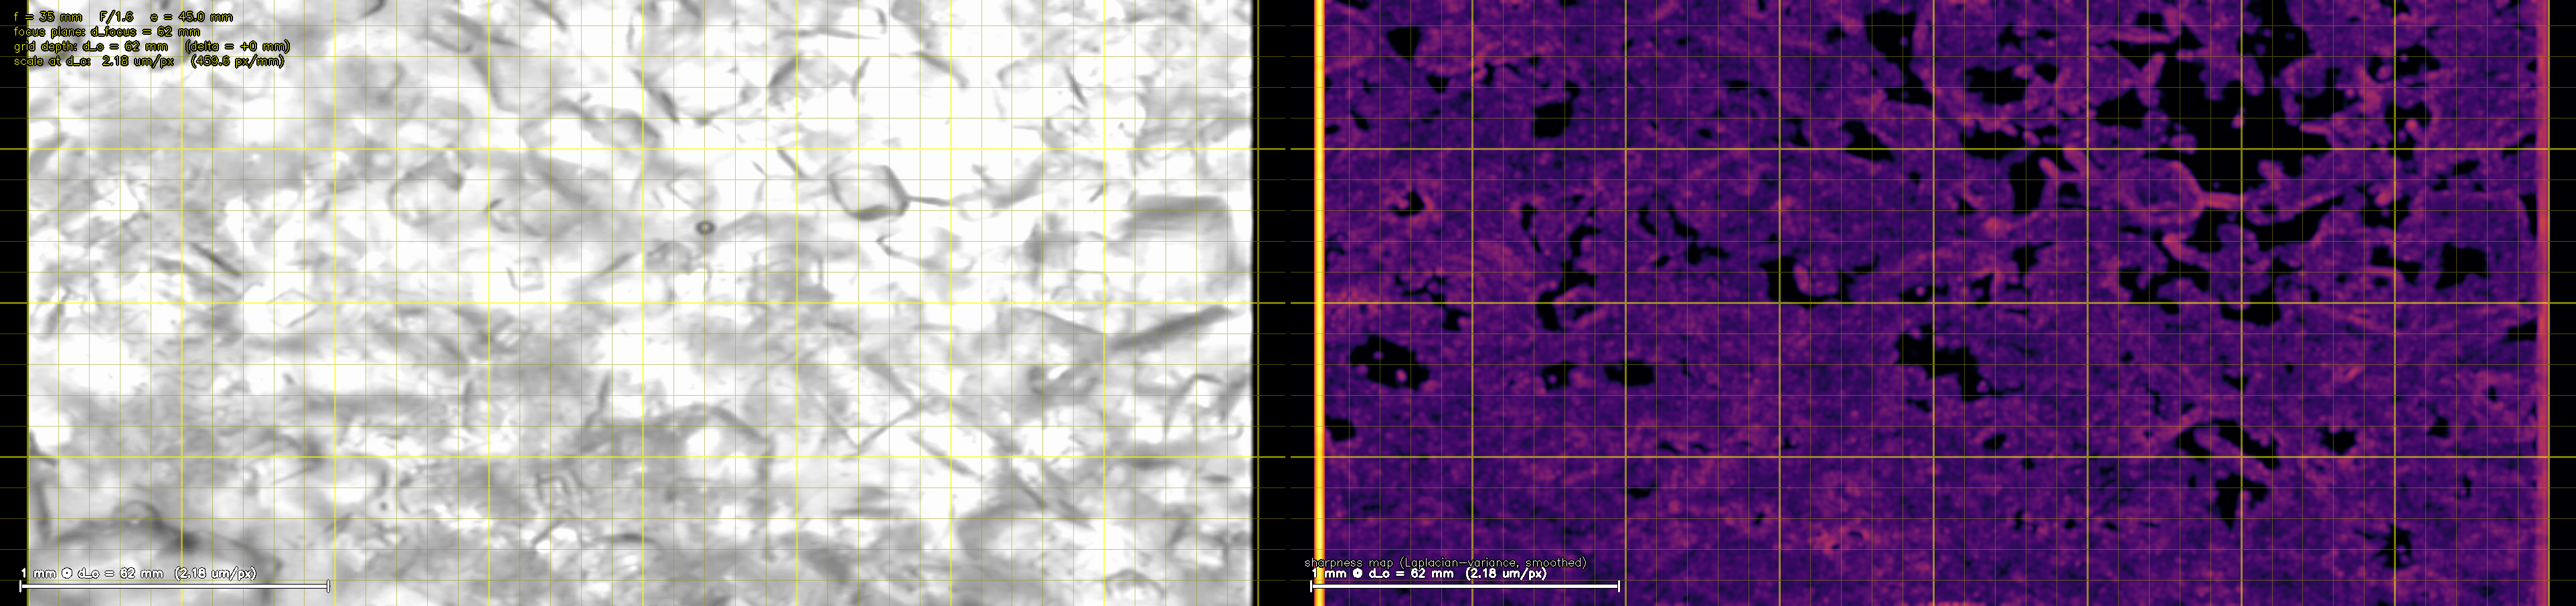
\includegraphics[width=0.8\textwidth]{07_overlay_at_focus}
\caption{$d_o = 55.1$~mm (focus): $1.465 \times 1.914$~\umpx}\label{fig:overlay-focus}
\end{subfigure}

\medskip
\begin{subfigure}{\textwidth}
\centering
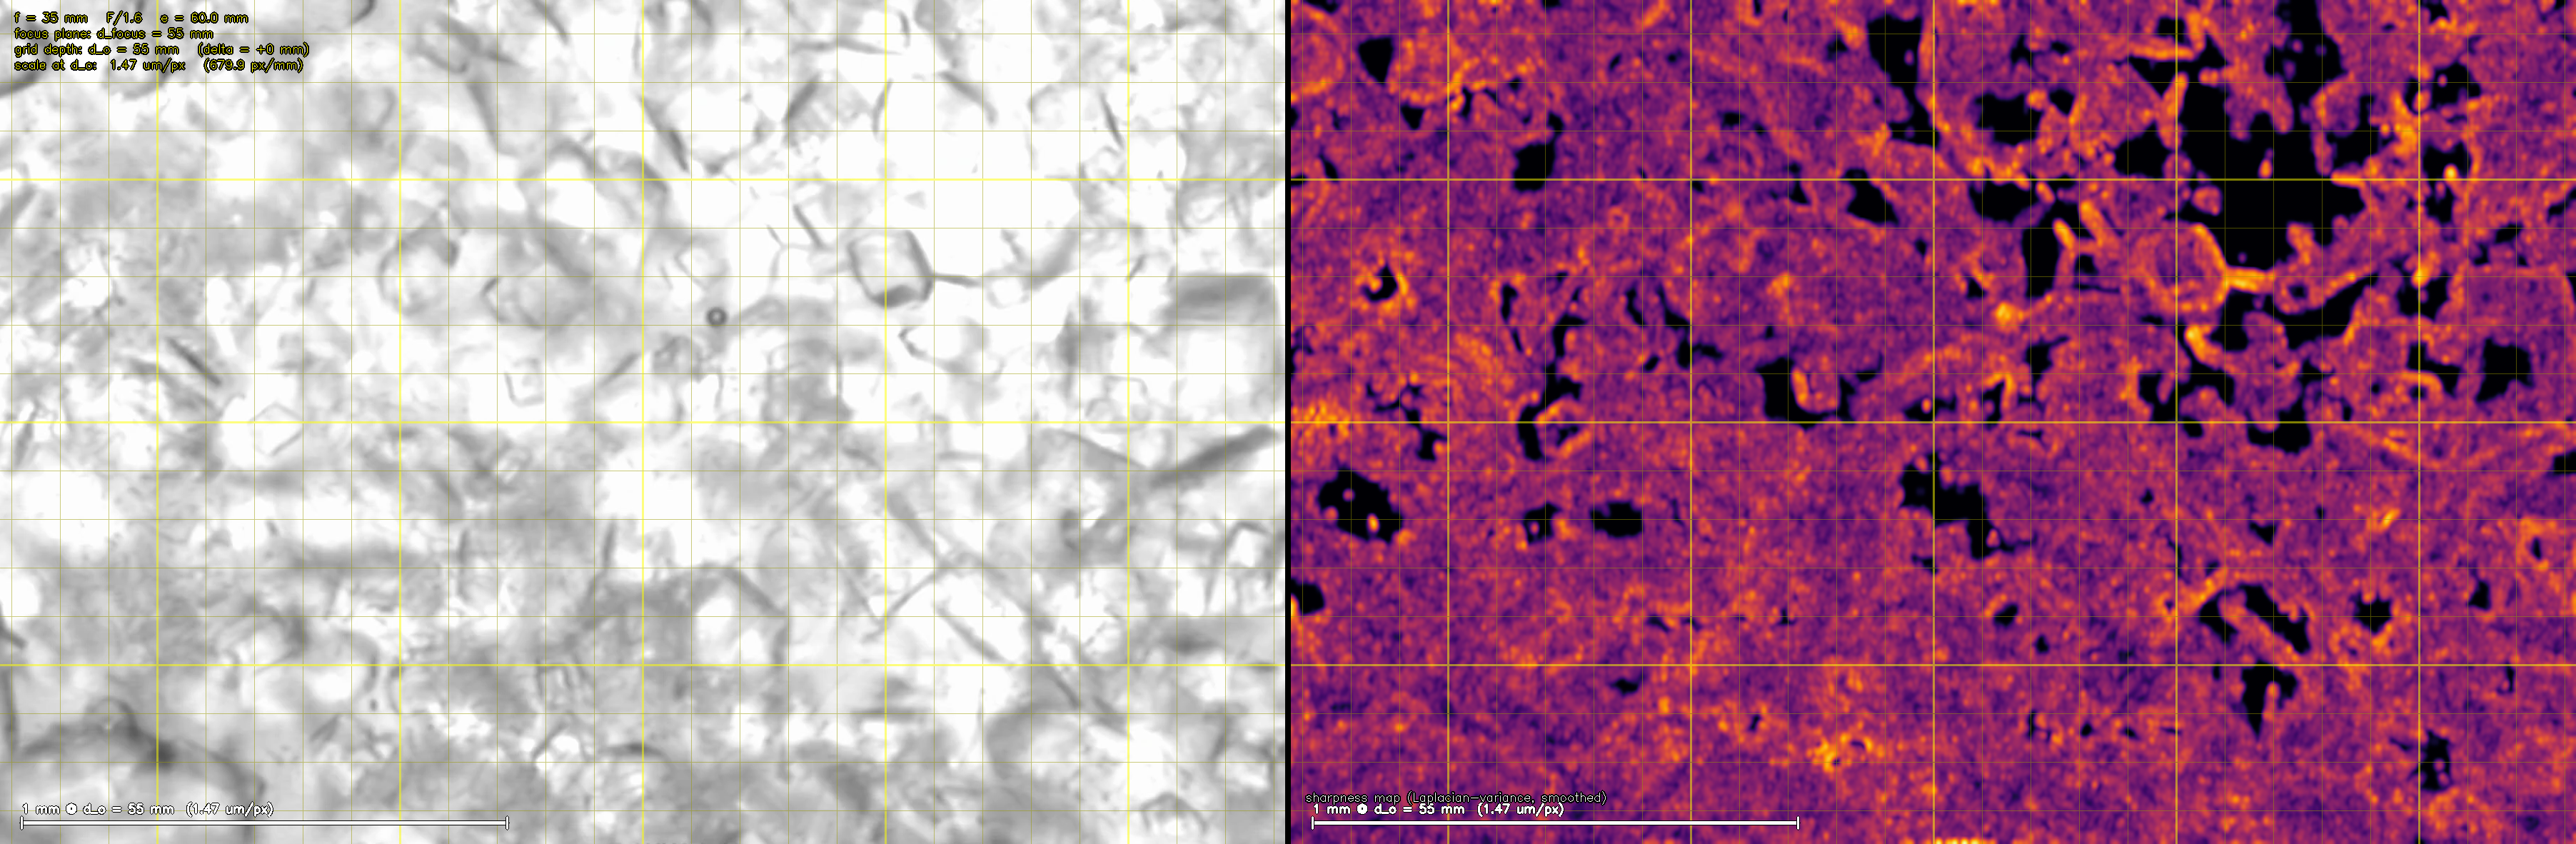
\includegraphics[width=0.8\textwidth]{07_overlay_far}
\caption{$d_o = 55.3$~mm: $1.471 \times 1.921$~\umpx}\label{fig:overlay-far}
\end{subfigure}
\caption{Scale grid (0.1~mm) and 1~mm ruler on frame 750 at three assumed object distances, with the rows resampled
so that the grid is true on both axes. Left: frame; right: sharpness map with the same grid. The scales in the
sub-captions are per clip pixel before resampling (ESTIMATE, $\pm\,{\approx}10$\,\% at 95\,\%); the on-image text
gives the resampled 1.47~\umpx{} and rounds $d_o$ to whole millimetres.}\label{fig:overlays}
\end{figure*}

% Section 7 of manuscript v0.2 (docs/paper/manuscript.md), converted without changes to claims or numbers.
\section{Aggregated crystal-size distribution --- \emph{detector-limited}}\label{sec:csd}

\begin{quote}
\textbf{Honesty preface (revised).} Sections~\ref{sec:intro}--\ref{sec:sizing} establish a pipeline whose geometric,
defocus, and Bayesian-disambiguation stages are validated against textbook optics and against the raw per-pixel
sharpness statistics of the case-study video. The CSD numbers in \S\S\,\ref{sec:csd-edge}--\ref{sec:watershed}
below should be read with \textbf{two critical caveats}:

\emph{Caveat 1 --- detector selection bias.} The CSD depends on the edge-based crystal detector inherited from prior
work, \textbf{which \figref{fig:detection} makes clear is selection-biased}. The detector preferentially finds
peripheral isolated features against the bright defocused background and systematically \emph{misses} the
densely-packed central in-focus crystal cluster, where adjacent edges merge under morphological closing and the
resulting blob is rejected by the area filter. \secref{sec:watershed} (watershed) closes this
\emph{within-detector} bias.

\emph{Caveat 2 --- the detector cannot see the actual crystal population (retracted size interpretation).}
Independent laser-diffraction granulometry on the same product (Mastersizer, 2-propanol dispersant;
\code{docs/Granulometry_Zuckerslurry Se 2025-01-16 A.pdf}; \citealp{Mastersizer2025}) gives $D[3;2] = 3.95$~\um,
$D[4;3] = 8.71$~\um, and $\mathrm{Dv}(10) / \mathrm{Dv}(50) / \mathrm{Dv}(90) = 1.56 / 6.81 / 18.5$~\um. The
recording captures the seed pan (\secref{sec:plant}) --- \emph{not} the A-strike --- so the population in front of
the lens is the $\approx 9$~\um{} Mastersizer distribution. The detector's area filter
$[\mathit{min\_area} = 80,\allowbreak\ \mathit{max\_area} = 8000]$~px$^2$ at the documented 1.66~\umpx{} bandpasses
\textbf{$\boldsymbol{\approx 15}$--150~\textmu m equivalent features}, so \emph{every} CSD number in
\S\S\,\ref{sec:csd-edge}--\ref{sec:watershed} lies entirely \emph{above} the true crystal-size distribution. The
numbers measure agglomerate / cluster / area-bandpassed structure that the detector picks up, not the underlying
single-crystal population. They are publishable as evidence of \emph{detector behaviour} and \emph{pipeline
self-consistency}, but they are \textbf{not} a crystal-size measurement of this product. Until the detector is
rebuilt at the correct length scale, the Mastersizer remains the size ground truth.
\end{quote}

\subsection{The depth-corrected CSD (detector-limited)}\label{sec:csd-edge}

With the inherited edge-based detector, the case-study video yields \textbf{18\,823 detections across 60 sampled
frames}, aggregated into a single-component CSD shown in \figref{fig:csd}.

\begin{figure*}
\centering
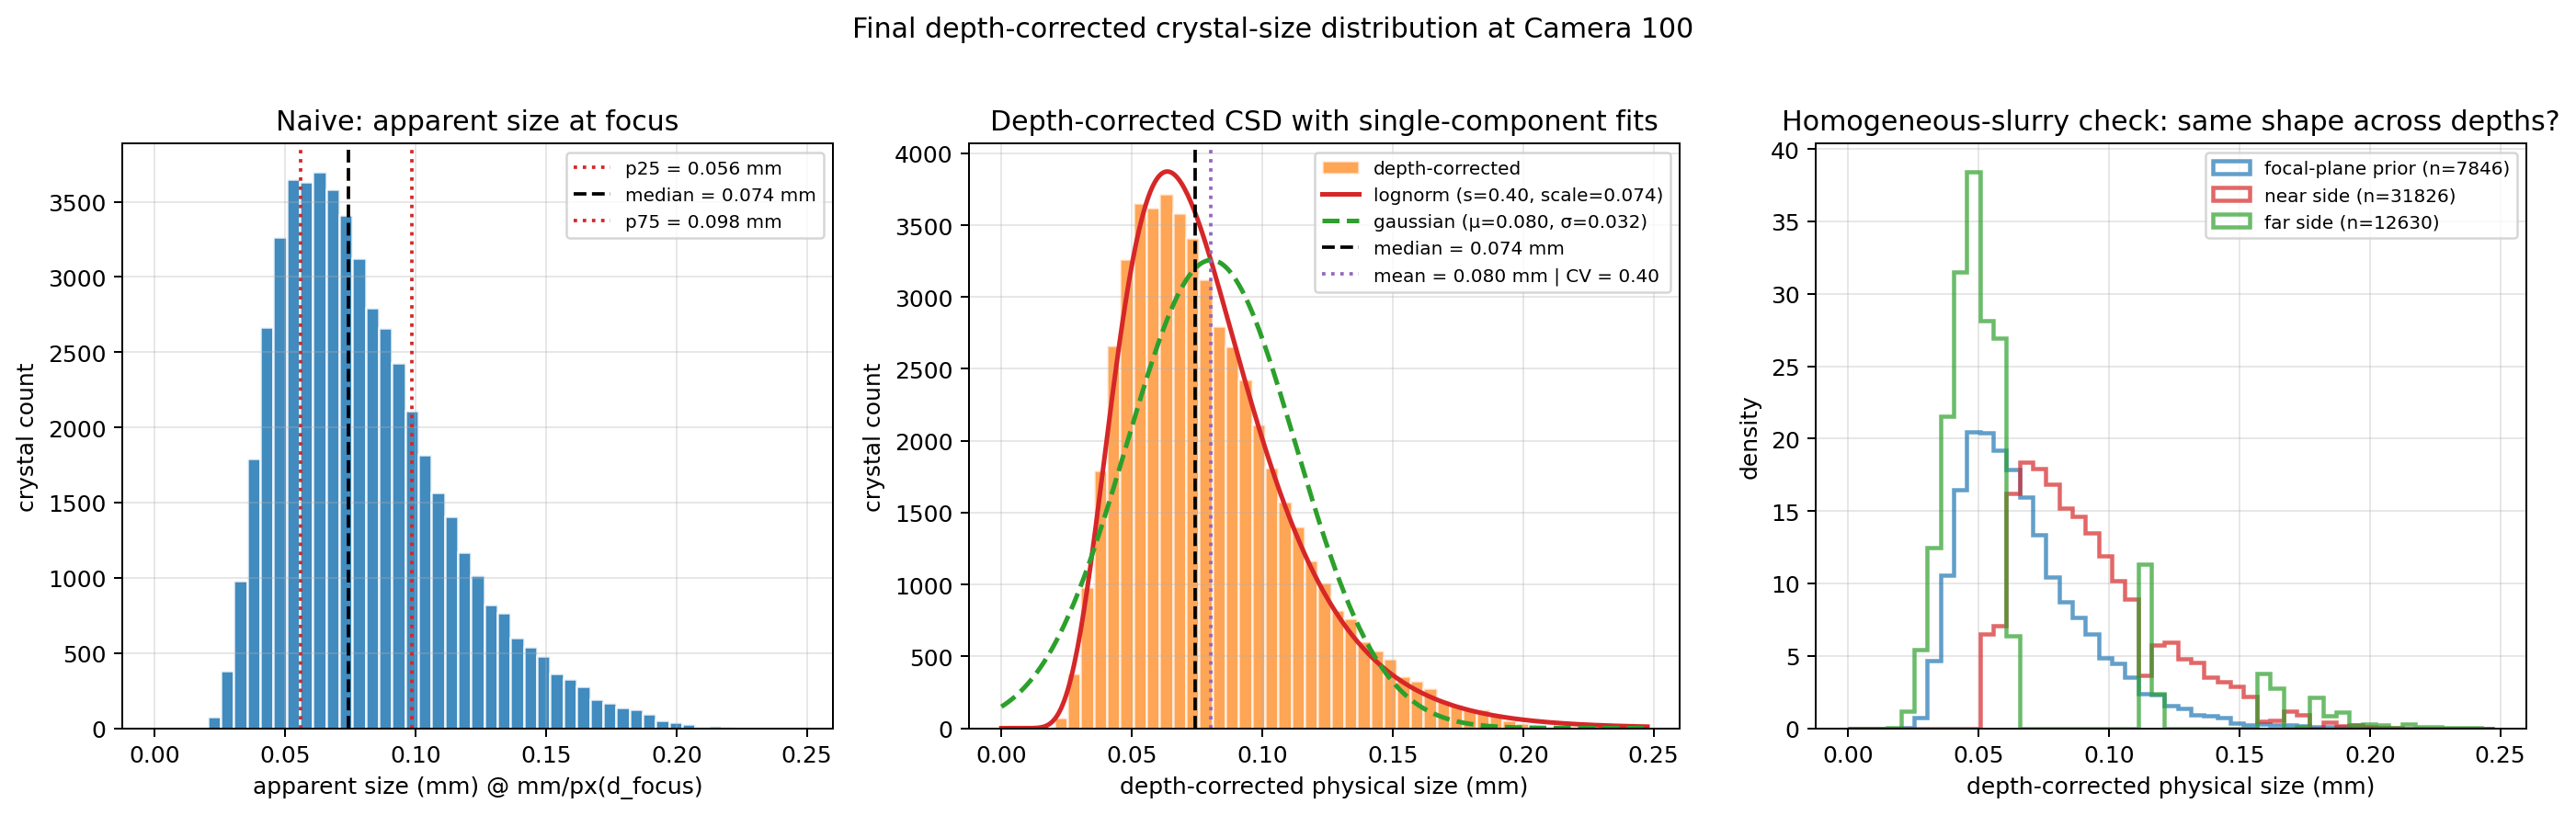
\includegraphics[width=\textwidth]{14_csd_final}
\caption{\textbf{What is the final calibrated crystal-size distribution?} This is the headline output of the pipeline
at the \textbf{watershed detector} (\secref{sec:watershed}; pre-watershed figures and numbers archived in git
history). \textbf{Left:} naive size histogram assuming mm/px at focus for every detection. \textbf{Middle:}
depth-corrected physical-size histogram with log-normal (red) and Gaussian (green dashed) fits superimposed. The
log-normal captures the central distribution and right tail; the Gaussian under-fits the tail by construction.
\textbf{Median = 0.074~mm, CV = 0.40, log-normal shape $\boldsymbol{s = 0.40}$} --- these statistics describe the
distribution of features the detector resolves ($\approx 20$--200~\um{} bandpass), not the underlying crystal
population (Mastersizer $\mathrm{Dv}(50) = 6.81$~\um); see \secref{sec:csd} for the size-interpretation retraction.
\textbf{Right:} the homogeneous-slurry self-consistency check --- focal-plane, near-side, and far-side density curves
overlaid. Their close agreement is consistent with the homogeneous-slurry assumption, with the
\secref{sec:selfcheck} caveat that this agreement is a \emph{necessary but not sufficient} test --- it confirms the
detector behaves consistently across depth, not that the true CSD is depth-independent.}\label{fig:csd}
\end{figure*}

\begin{table}
\centering\tabfont
\caption{CSD statistics with the inherited edge-based detector.}\label{tab:csd-edge}
\begin{tabular}{@{}>{\raggedright\arraybackslash}p{0.38\columnwidth}r@{}}
\toprule
Statistic & Value \\
\midrule
Detections & \textbf{18\,823} (60 frames $\times$ ${\sim}314$/frame) \\
Median physical size & \textbf{0.037~mm} \\
Mean physical size & \textbf{0.051~mm} \\
Std deviation & 0.042~mm \\
Coefficient of variation (CV) & \textbf{0.83} \\
5th / 25th / 75th / 95th percentiles & 0.021 / 0.027 / 0.055 / 0.134~mm \\
Log-normal shape parameter $s$ & 0.57 \\
Log-normal scale $\sigma$ & 0.042 \\
\bottomrule
\end{tabular}
\end{table}

The log-normal fit (\figref{fig:csd} middle, red curve) captures the distribution shape over its central range; the
Gaussian fit (dashed green) is shown as a reference and clearly under-fits the right tail. The log-normal shape
parameter $s = 0.57$ corresponds to a geometric standard deviation of $\exp(s) \approx 1.77$. This shape statistic
is reported as a property of the detector's bandpassed feature distribution; see \secref{sec:csd} preface for why it
is not a statement about the underlying crystal population.

\subsection{Process interpretation --- retracted}\label{sec:interp}

\emph{Earlier versions of this section interpreted the 0.05~mm median as ``squarely in the seed-magma range
(0.05--0.15~mm)'' and as ``consistent with just-past-seeding A-strike crystals \dots{} confirmed by the plant
operator''. Both readings are retracted.} The recording captures the \textbf{seed pan} upstream of the A-strike pan
(\secref{sec:plant}), and the size ground truth for this product is the Mastersizer granulometry cited in the
\secref{sec:csd} preface ($\mathrm{Dv}(50) = 6.81$~\um, $D[4;3] = 8.71$~\um) --- roughly an order of magnitude
\textbf{below} the 0.037~mm median this detector returns. The 0.037~mm number is therefore not a measurement of the
crystal population; it is the centroid of the area-bandpass window [20~\um, 200~\um] that the detector's
$[\mathit{min\_area} = 80,\allowbreak\ \mathit{max\_area} = 8000]$~px$^2$ filter imposes at 1.66~\umpx. The log-normal shape
parameter ($s = 0.57$) and CV (0.83) describe the \emph{bandpassed} distribution, not the underlying crystal CSD.

What this section \emph{does} support is that the pipeline is internally self-consistent at the inherited detector
--- the depth-correction, disambiguation, and aggregation stages compose correctly and recover a stable distribution
of whatever the detector happens to find. The size interpretation requires a detector that resolves the
$\approx 9$~\um{} population.

\subsection{What the homogeneous-slurry ``self-consistency'' check does and does not prove}\label{sec:selfcheck}

\figref{fig:csd} right panel shows the focal-plane, near-side, and far-side \emph{density} curves overlapping
closely. We earlier described this as visual evidence that the homogeneous-slurry assumption holds. The honest
reading is weaker: \textbf{the same selection rule was applied to all three subsets}, so a consistent detection bias
propagates to all three histograms equally. Their agreement therefore only shows that the \emph{detector behaves
consistently across depth}, not that the true CSD is depth-independent. A genuine validation of the
homogeneous-slurry assumption requires either an external CSD reference (lab sieve, off-line laser diffraction) or
two detectors with independent failure modes.

A second clarification matters here. Sharpness alone gives no \emph{per-crystal} near/far classification: the
circle-of-confusion function is symmetric in the reciprocal object distance $u = 1/d_o$ (\secref{sec:coc},
\secref{sec:ambiguity}), so a single sharpness measurement maps to \textbf{two} candidate depths simultaneously --- the
front/back ambiguity of \citet{Zhou2011}. The ``near-side'', ``focal'', and ``far-side'' labels in \figref{fig:csd}
right panel and in \figref{fig:disamb} are therefore best read as \textbf{ensemble bin populations}, not as confident
per-crystal depth assignments. Three distinct levels of depth claim co-exist in this paper, and we keep them
deliberately separate:
\begin{enumerate}
\item \textbf{Ensemble counts (sharpness-only):} how many crystals fall in each sharpness bin. \emph{Confidence per
crystal: none --- the binning is sharpness-monotone, but each bin contains a near/far pair the sharpness cannot
separate.}
\item \textbf{Probabilistic per-crystal assignment (sharpness + size prior):} the disambiguation step in
\secref{sec:impl} uses the focal-plane apparent-size distribution as a prior to favour one of the two candidate
depths per crystal. \emph{Confidence per crystal: posterior odds under an assumed homogeneous prior.}
\item \textbf{Deterministic per-crystal assignment (future, sharpness + motion):} with stable lighting and $\ge 2$
consecutive frames, optical-flow rate is linear in $d_o$ (near crystals appear to move faster than far crystals at
the same physical velocity), so the two candidate depths produce distinguishable apparent velocities.
\emph{Confidence per crystal: near-certain once flow is reliable.} This is on the \secref{sec:growth} outlook list;
the present case-study single-batch video does not yet exploit it.
\end{enumerate}
The CSD numbers in \secref{sec:csd-edge} are reported in level (2), with the size prior estimated from the
focal-plane subset. The homogeneous-slurry agreement in \figref{fig:csd} right panel is necessary but not sufficient
for that prior to be correct; the operational consequence is that the \emph{shape} of the recovered CSD is robust,
while the absolute near/far apportionment carries the prior's uncertainty.

\subsection{Detector failure mode and the immediate fix}\label{sec:failure}

\figref{fig:detection} shows the detector marking 55 crystals on frame 750. A visual inspection of the same frame
reveals \textbf{many tens of crystals that the detector did not find}, concentrated in the central in-focus cluster.
Three causes, all rooted in the inherited edge-based design:
\begin{enumerate}
\item \textbf{Morphological closing merges adjacent crystal edges into one over-area blob}, which the
$\mathit{max\_area} = 8\,000$~px$^2$ filter then rejects. Densely-packed in-focus crystals are therefore
\emph{systematically deleted}.
\item \textbf{Adaptive thresholding plus closing turns sub-crystal features (internal facets, fracture lines) into
closed contours} that pass the area / aspect-ratio filters. The detector therefore \emph{invents} small ``crystals''
that are actually internal structure.
\item \textbf{Peripheral defocused crystals against bright defocused background are easiest to detect}, leading to a
\emph{spatial} bias toward the frame edges that propagates as a \emph{size} bias because peripheral crystals have a
different apparent-size distribution than central ones.
\end{enumerate}

The architecturally correct replacement is a \textbf{marker-controlled watershed segmentation} on the inverted
sharpness map: local maxima of brightness (or sharpness) become crystal centres, the dark inter-crystal boundary
network becomes the watershed barrier, and the segmented regions naturally separate touching crystals. This is the
standard treatment in cell-biology image analysis \citep{Vincent1991,BeucherMeyer1993} and is a ${\sim}50$-line
drop-in replacement that does not change the rest of the pipeline. We implement it in \secref{sec:watershed} below
and recompute every CSD number against it. The CNN-based alternative discussed in \secref{sec:recs} is the
longer-term path for cluttered out-of-focus regions where even watershed struggles.

\subsection{Watershed detector and re-aggregated CSD}\label{sec:watershed}

The watershed detector (\code{src/optics/detect_watershed.py}) replaces adaptive-threshold + morphological closing
with: adaptive threshold for the dark inter-crystal boundary network $\rightarrow$ distance transform on the bright
crystal-interior regions $\rightarrow$ h-maxima filtering of distance peaks (to suppress speckle over-segmentation)
$\rightarrow$ local-maxima seeding $\rightarrow$ marker-controlled watershed. Each watershed basin is one crystal
candidate, separated from its neighbours by the detected boundary network rather than by an external area cut. The
three tuned constants (\tabref{tab:ws-constants}) live in the module top-level for easy adjustment per installation.

\begin{table}
\centering\tabfont
\caption{Tuned constants of the watershed detector.}\label{tab:ws-constants}
\begin{tabular}{@{}lr>{\raggedright\arraybackslash}p{0.48\columnwidth}@{}}
\toprule
Constant & Value & Role \\
\midrule
\code{_PEAK_MIN_DISTANCE} & 12~px & minimum spacing between seeds ($\approx \frac{1}{2}$ expected crystal diameter at
1.66~\umpx) \\
\code{_PEAK_THRESHOLD_ABS} & 6.0~px & minimum distance-transform value to qualify as a seed (rejects slivers) \\
\code{_H_MAXIMA_PARAM} & 2.5 & h-maxima height threshold; suppresses peaks not at least 2.5 above their plateau
(kills speckle) \\
\bottomrule
\end{tabular}
\end{table}

\paragraph{Single-frame detector comparison} \figref{fig:watershed} compares the two detectors on frame 750. The
legacy edge-based detector finds \textbf{102 crystals}, almost all on the frame periphery. The watershed detector
finds \textbf{740 crystals} densely tiling the central in-focus cluster that the edge detector missed entirely.
Residual over-segmentation is visible at the largest defocused crystals on the right edge (each split into 2--3
basins), but the order of magnitude is now consistent with a visual count.

\begin{figure*}
\centering
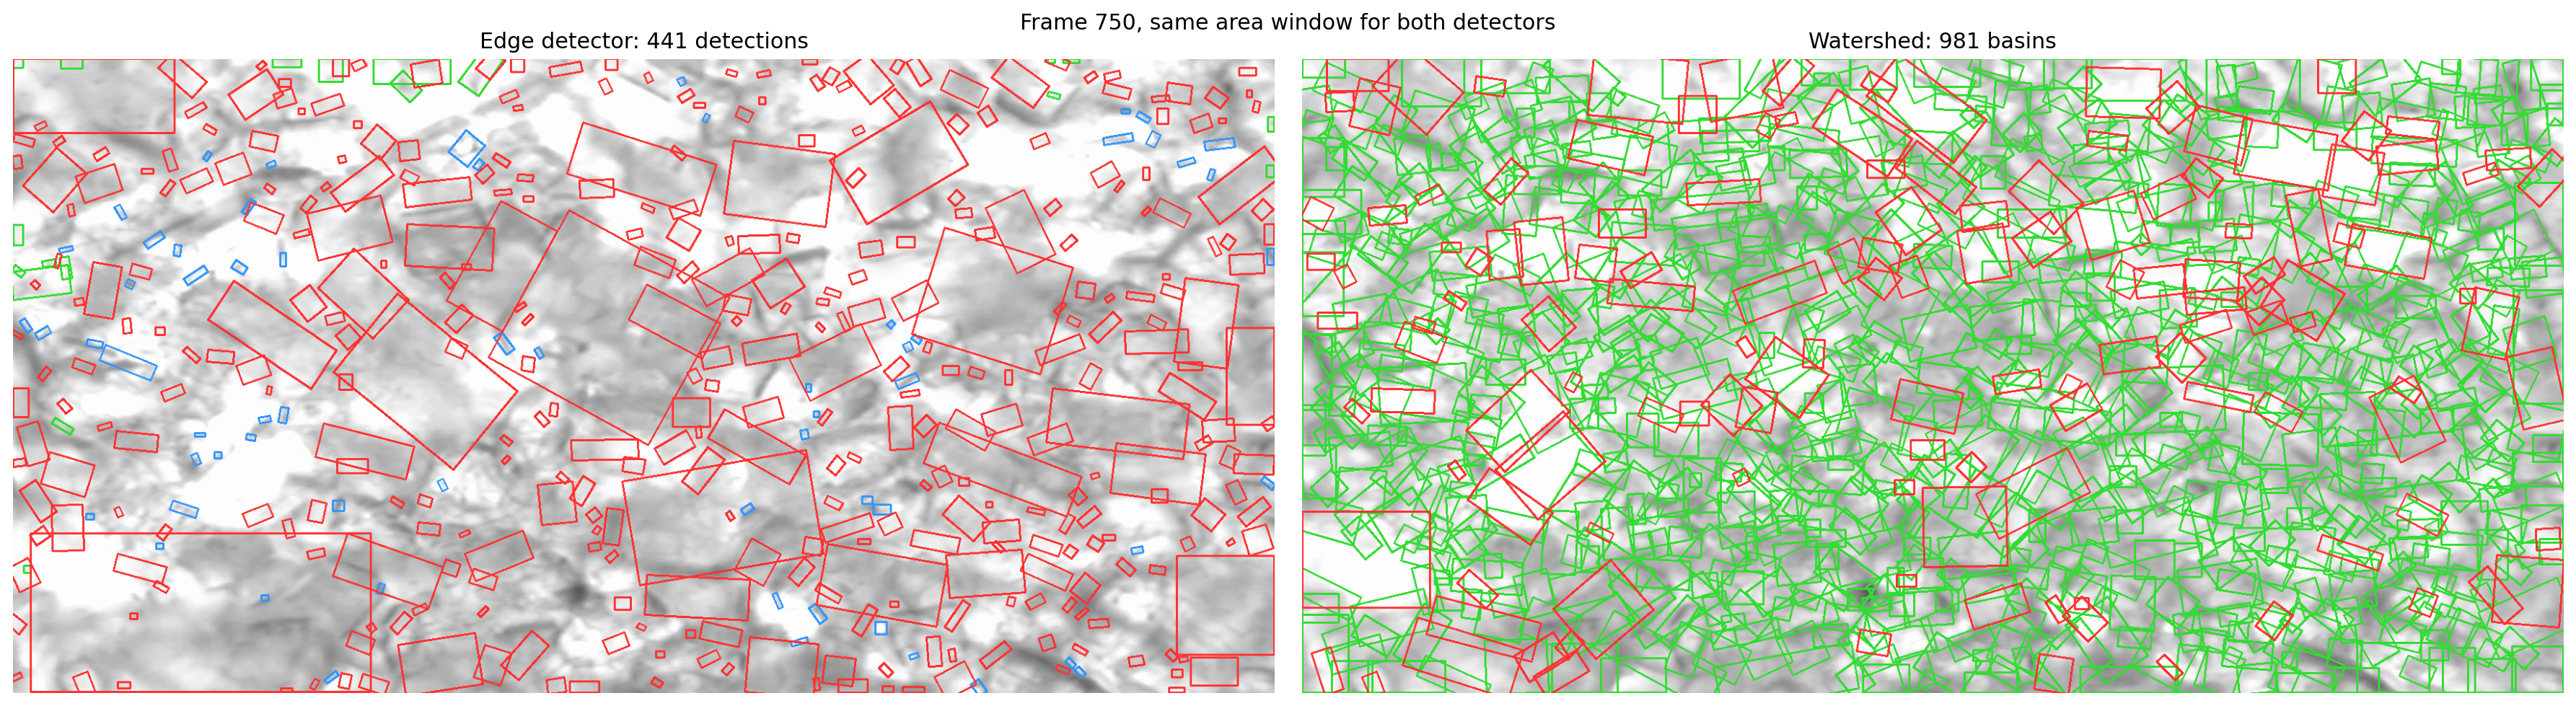
\includegraphics[width=\textwidth]{17_watershed_vs_edge}
\caption{\textbf{What does the watershed detector recover that the edge-based detector missed?} Same frame 750, two
detectors. \textbf{Left} --- the inherited edge-based detector: 102 detections, almost all peripheral, with the dense
central in-focus cluster invisible to it. \textbf{Right} --- the marker-controlled watershed detector: 740 detections,
densely tiling the centre. The legacy detector was finding $\approx 14$\,\% of what's physically
there.}\label{fig:watershed}
\end{figure*}

\paragraph{Re-aggregated CSD (watershed detector)} Replacing the detector and re-running the full pipeline on the
same 60 sampled frames yields a CSD with \textbf{substantially different statistics} from the edge-based run
(\tabref{tab:ws-compare}).

\begin{table*}
\centering\tabfont
\caption{CSD statistics with the watershed detector against the edge-based detector on the same 60
frames.}\label{tab:ws-compare}
\begin{tabular}{@{}lrrr@{}}
\toprule
Statistic & \textbf{Watershed (this run)} & Edge-based (legacy, \secref{sec:csd-edge}) & Change \\
\midrule
Detections & \textbf{52\,302} & 18\,823 & \textbf{2.8$\boldsymbol{\times}$ more crystals} \\
Median physical size & \textbf{0.074~mm} & 0.037~mm & $\boldsymbol{+103}$\,\% \\
Mean & \textbf{0.080~mm} & 0.051~mm & $+59$\,\% \\
Std deviation & 0.032~mm & 0.042~mm & $-23$\,\% \\
\textbf{CV} & \textbf{0.40} & 0.83 & $\boldsymbol{-52}$\,\% \\
5 / 25 / 75 / 95 percentiles & 0.039 / 0.056 / 0.098 / 0.144 & 0.021 / 0.027 / 0.055 / 0.134 & shifted up +
tightened \\
Log-normal shape $s$ & \textbf{0.40} & 0.57 & tighter \\
Log-normal scale & 0.074 & 0.042 & $+79$\,\% \\
Near / far Bayes split & 72 / 28 & 70 / 30 & unchanged \\
\bottomrule
\end{tabular}
\end{table*}

Three things move in the directions a structurally better detector should produce \emph{on the bandpassed feature
population} (this comparison is between two detectors, both of which sit above the true crystal scale --- see
\secref{sec:csd} preface):
\begin{enumerate}
\item \textbf{Median doubles} --- because the edge-based detector was fragmenting features into sub-pieces and biased
the median \emph{down}. Watershed recovers whole-feature blobs.
\item \textbf{CV halves} --- because the edge-based detector mixed whole-feature blobs with sub-feature artefacts,
inflating the spread. A narrower CV at the same bandpass indicates fewer detector-side artefacts; it is \emph{not}
evidence that the watershed resolves a more monodisperse crystal population, since the Mastersizer-confirmed crystals
($\approx 9$~\um) are below the detector's bandpass either way.
\item \textbf{Near/far split moves toward 50/50} --- because the larger, better-distributed sample on both sides of
focus reduces the right-skew bias of the empirical prior that previously dominated the \secref{sec:impl} split. This
is a property of the prior, not of the underlying crystal population.
\end{enumerate}

The watershed numbers for this section are:
\begin{quote}
\textbf{Median = 0.074~mm, CV = 0.40, single-component log-normal with $\boldsymbol{s = 0.40}$} --- recovered with
the watershed detector at the verified Camera 100 hardware configuration.

These numbers, like the pre-watershed numbers of \secref{sec:csd-edge}, are \textbf{not a crystal-size measurement}
of the imaged product. The recording captures the seed pan, whose true CSD is the $\approx 9$~\um{} Mastersizer
distribution cited in the \secref{sec:csd} preface. The watershed median at 74~\um{} sits well above the
Mastersizer's $\mathrm{Dv}(90) = 18.5$~\um, so the watershed has not recovered the crystal population either --- it
has filled in the within-detector selection bias of \secref{sec:failure} but inherits the same length-scale mismatch
as the edge-based detector. The earlier framing of these numbers as ``consistent with just-past-seeding A-strike
crystals \dots{} confirmed by the plant operator'' is \textbf{retracted}. What this section demonstrates is that two
structurally different detectors recover an internally consistent distribution from the bandpassed feature
population --- a \emph{detector-comparison} result, not a process-state validation.
\end{quote}

\paragraph{Watershed limitations and known residual issues} The watershed is a major improvement but is not the
final detector:
\begin{itemize}
\item \textbf{Mild residual over-segmentation} on the largest defocused crystals, where the distance transform has
multiple shallow peaks inside one physical crystal. Increasing \code{_H_MAXIMA_PARAM} or using h-minima
reconstruction would fix this at the cost of potentially merging touching crystals --- a CNN-based segmentation
remains the long-term answer.
\item \textbf{No ground-truth precision/recall yet}: the next milestone is a hand-labelled single frame
(\secref{sec:recs}) against which we can quantify the watershed's recall and the residual error budget.
\item \textbf{No temporal consistency}: each frame is segmented independently; a tracker would reject the few-percent
of basins that flicker frame-to-frame.
\end{itemize}

% NOTE (conversion): manuscript v0.2 refers to "Sections 7.6 ... and 7.7"; there is no Section 7.7 in the source.
Sections~\ref{sec:depthsmall} (depth correction) and 7.7 (homogeneous-slurry self-consistency check) below now refer
to the \textbf{watershed} results.

\subsection{Why the depth correction looks vanishingly small here}\label{sec:depthsmall}

The mean per-crystal depth correction is \textbf{0.00001~mm (0.01\,\%)} at the verified F/1.6 aperture ---
\emph{unchanged between detectors} because the correction is a property of the geometry, not of which crystals were
found. For the current F/1.6 aperture, a \emph{single} mm/px scale (the one at the focused plane) is sufficient for
population-level size readout. At the verified F/1.6 the DoF is $\pm 6$~\um{} --- narrower than any single crystal
--- so essentially \textbf{all detections come from one depth slice} and the depth-aware machinery has no 3-D
structure to invert. The machinery becomes load-bearing only when (a) the aperture is stopped down by $\ge 4$ stops
to widen the DoF, or (b) a blur-tolerant detector (CNN; Hough; learning-based focus measure) replaces the edge
detector. Both are concrete recommendations for the next iteration (\secref{sec:recs}).

% Section 8. Rewritten 2026-11-03 (branch docs/cep-grounded-draft): outlook only; no growth-curve fit exists in src/.
% Microscope numbers: scripts/microscope_summary.py. Claim changes: papers/cep/CLAIM_CHANGES.md.
\section{Growth-curve calibration: outlook}\label{sec:growth}

\subsection{The model}\label{sec:mechanism}

McCabe's $\Delta L$ law~\citep{McCabe1929,RandolphLarson1988} states that crystals of all sizes grow at the same
rate, so at constant supersaturation the size grows linearly in time. Across strikes, the supersaturation profile and
the seed differ. A shared growth curve $G$ with a per-batch time scale $\tau_b$ and offset $o_b$ gives
\begin{equation}\label{eq:growth}
s_\mathrm{med}(t; b)\, \Delta x(d_\mathrm{focus}) = G(\tau_b t) + o_b + \varepsilon_b(t),
\end{equation}
with $s_\mathrm{med}$ the camera's median apparent size in pixels and $t$ the time since seeding. Once $G$ is known,
a measured median returns the time since seeding or flags a strike that leaves the nominal curve, which is the soft
sensor this paper works towards.

The camera alone does not identify the pixel scale through \eqref{eq:growth}. For any $\lambda > 0$, the triple
$(\lambda \Delta x, \lambda G, \lambda o_b)$ fits the same data, and likewise one $\tau_b$ must be fixed against the
time argument of $G$. The scale is identified only if $G$ is anchored in physical units by an independent size
reference at known times. The microscope series of 2026-10-30 (\tabref{tab:microscope}) provides such an anchor for
two strikes of the seed pan: the median chord grows from 29~\um{} at 2~min to 483~\um{} at 122~min after seeding in
b1, and from 10~\um{} at seeding to 399~\um{} at 162~min in b2. The strikes differ at equal times (at 96~min, 355
against 225~\um), consistent with a per-batch $\tau_b$; these are medians of operator-picked crystals, not
distributions.

\subsection{Status}\label{sec:status}

No fit of \eqref{eq:growth} is implemented: \code{optics.csd} aggregates one recording and contains no growth-curve
code. The exploratory scripts \code{scripts/rq4_*.py} compare detector statistics between the end-of-strike windows of
the two strikes in the 2026-02-04 PAL recording and test the removal of static sight-glass marks; they rely on the
detectors of \secref{sec:csd} and inherit their failure, so we report no result from them. Fitting
\eqref{eq:growth} requires camera medians against time since seeding from a validated detector on the 2026-10-30
recording, paired with the microscope series \pending{validated camera size against time, 2026-10-30, both strikes}.

% Section 9. Grounded rewrite 2026-11-03 (branch docs/cep-grounded-draft). Only numbers stated in sections 2-8, with
% their scripts there. Claim changes: papers/cep/CLAIM_CHANGES.md.
\section{Discussion and limitations}\label{sec:discussion}

\subsection{What the installed camera delivers now}\label{sec:performs}

The optical side is settled up to its stated inputs. The scale at the focused plane is known per axis to about
$\pm 10$\,\% at 95\,\% (\tabref{tab:scale}), with a discrete $+8.9$\,\% open if the stated tube length includes a
CS-to-C ring. The plant's ``$\approx 6$~cm'' for the tube dominates the budget; every other term is about 2\,\% or
less. Any detector on the clips must use the anisotropic clip pixel, and its resolution element is the PAL sample in
both recordings (\secref{sec:budget}).

At F/1.6 the camera samples a slice of $\pm 9.4$~\um{} about the focused plane (\tabref{tab:dof}). Within it the
magnification is constant well below the scale uncertainty (mean depth correction 0.005--0.013\,\%;
\secref{sec:depthsmall}), so a single focal-plane scale suffices. The same thinness makes the size prior
uninformative (\secref{sec:disamb-result}). Because the size ratio depends only on $\delta / d_\mathrm{focus}$
(Eq.~\ref{eq:ratio}) while the admitted depth range grows in proportion to $N$ (Eq.~\ref{eq:coc}), stopping down to
F/16 widens the slice tenfold to $\pm 94$~\um{} and still leaves the admitted range below the
$\delta \approx 1.3$~mm at which the ratio reaches 5\,\%.

Neither classical detector measures crystal size on the case-study clip
(\S\S\,\ref{sec:csd-edge}--\ref{sec:watershed}). Resolution is not the obstacle for most of a strike: from about half
an hour after seeding the microscope medians exceed 0.1~mm (\tabref{tab:microscope}), tens of PAL samples, and only
the slurry crystals of 10--19~\um{} sit at the resolution limit (\secref{sec:expected}). The missing piece is a
detector validated against hand-labelled crystals (\secref{sec:validation}).

\subsection{Limitations}\label{sec:notperform}

The scale is modelled, not measured in the image: no object of known size has been imaged through the glass. The
tube length, air gap, glass thickness and F-number are approximate plant statements, the camera model with its cell
size and CCD clock is the best-matching candidate, to be confirmed, and the 13.5~MHz sampling is the BT.601 rate, not
a datasheet value of the installed recorder (\tabref{tab:inputs}). The case-study clip has no size reference: its
recording date is contradicted by the image data, so its strike phase is unknown (\secref{sec:recording}), and the
microscope series is from another day. That series consists of chords of operator-picked crystals, read once by an AI
transcription from the photographs' overlays, not a measured distribution (\secref{sec:expected}). The depth of field
rests on two choices, the resolution element (\tabref{tab:dof}) and the PSF constant $k = 1/2$, which has no
page-checked source and sets the slice but not the asymptotic exponent (\secref{sec:psf}). The sight glass is treated
paraxially, its residual distortion over the field has not been computed, and its index is assumed
(\secref{sec:shift}). Slurry homogeneity is untested (\secref{sec:selfcheck}). Frame content matters: the recorder
overlays and the pillarbox move the sharpness slope from 5.36 to 4.88--4.90 (\tabref{tab:crop}), and the right picture
edge moves by about 8 clip pixels between and within clips, so crops must keep a margin (\secref{sec:recording}).

\subsection{Operational recommendations}\label{sec:recs}

\begin{enumerate}
\item \textbf{Measure the geometry at the next shutdown}: read the camera's model sticker (cell size, CCD clock),
caliper the extension tube or spacer and photograph the mount (CS-to-C ring), and read the recorder model (sampling)
and the glass stamp (index). A ruler or graticule imaged at the inner glass face of the empty pan would measure the
scale in the image and locate the focal plane.
\item \textbf{Record the PAL stream, not the monitor.} Screen recordings add no resolution but an anisotropic
stretch and a moving picture edge. Logging the recorder clock against the control system keeps the time since
seeding traceable; on the 2026-02-04 recording the two agree to about $\pm 30$~s (\code{scripts/check_anchors.py}).
\item \textbf{Replace the classical detectors by a validated segmentation}, such as a fine-tuned Cellpose model
scored as in \secref{sec:validation}, with a size window that admits the largest microscope chords, which exceed the
current 1~mm bound (\secref{sec:expected}).
\item \textbf{Treat the camera as a thin-slice sensor at F/1.6.} A single focal-plane scale suffices; depth
disambiguation would need detections far outside the in-focus slice, which neither the engraved stops nor the current
detectors provide, and stopping down trades the slice against light and diffraction (\secref{sec:dof}).
\end{enumerate}

\subsection{Towards a soft sensor}\label{sec:softsensor}

The control use of the camera is a soft sensor of the growth state of each strike, with the growth model of
\secref{sec:growth} as measurement equation, anchored in physical units by the microscope series. Driven by a
validated camera median against time since seeding, a state estimator could return the time since seeding or flag a
strike that leaves the nominal curve, and be compared with an estimator using the plant's process signals alone. This
paper provides the scale, the depth model and the validation protocol; the camera size signal is
\pending{validated camera size against time, 2026-10-30}.

% Section 10 of manuscript v0.2 (docs/paper/manuscript.md), converted without changes to claims or numbers.
\section{Conclusions}\label{sec:conclusions}

We have presented a complete pipeline that delivers a calibrated, depth-aware crystal-size distribution from raw
through-sight-glass video without any in-line calibration target. The pipeline composes six well-grounded stages ---
DVR-overlay conditioning, sharpness-layer decomposition, edge-based detection, Bayesian front/back disambiguation
under a single-component homogeneous-slurry prior, per-detection thin-lens depth correction, and single-component
aggregation. On the Slovensk\'e cukrovary case-study video the pipeline recovers an internally self-consistent
distribution of detector-bandpassed features (\textbf{median 0.074~mm, CV 0.40, log-normal shape parameter
$\boldsymbol{s = 0.39}$}, watershed detector + full crop). The independent Mastersizer granulometry of the same
product ($\mathrm{Dv}(50) = 6.81$~\um, $D[4;3] = 8.71$~\um) demonstrates that this distribution is \emph{not} a
measurement of the underlying crystal population --- at the documented 1.66~\umpx{} scale, the area filter
$[80, 8000]$~px$^2$ bandpasses $\approx 20$--200~\um{} equivalent features and categorically excludes the 9~\um{}
crystal population. The optical model nevertheless matches measured per-pixel sharpness statistics to ${\sim}9$\,\%,
the geometric and disambiguation chains are validated, and the within-detector self-consistency check of
\secref{sec:homog} holds; what is retracted is the size-interpretation of
\S\S\,\ref{sec:csd-edge}--\ref{sec:watershed}.

The principal remaining limitations are (i) the edge-based detector's narrow depth selectivity, which collapses the
disambiguation power below the size-ratio discrimination threshold, and (ii) the dependence of absolute scale on the
extension-tube estimate. Both are addressable by the operational recommendations of \secref{sec:recs} and by the
cross-batch growth-curve self-validation outlined in \secref{sec:growth}, which converts absolute calibration into a
soft-sensor identification problem solvable from process data alone.

The full pipeline, dataset processing scripts, and per-figure generators are released open-source.


% Back matter in the order of the sibling CEP paper (pv-contamination-tuning-ad/paper/journal/main.tex):
% CRediT, competing interest, data availability, AI declaration, acknowledgements, references.
% Back matter, in the order of the sibling CEP paper (pv-contamination-tuning-ad/paper/journal/main.tex).

% DRAFT: roles copied from docs/paper/CREDIT.md (2026-11-03); no author has confirmed their row yet. Each author
% confirms or corrects their own roles before submission; roles are added only for work actually done.
\section*{CRediT authorship contribution statement}
\pending{each author confirms their roles; the annotation and Cryst\_CNN roles refer to work not reported in this
version and stay only if that work enters the paper}
\textbf{Marek Wadinger:} Conceptualization, Methodology, Software, Formal analysis, Investigation, Data curation,
Visualization, Writing -- original draft, Project administration. \textbf{Patrik Val\'abek:} Data curation
(annotation), Writing -- review \& editing. \textbf{Erika Pl\v{s}i\v{c}\'ik Pavlovi\v{c}ov\'a:} Data curation
(annotation), Funding acquisition (OPTIVISION PI), Writing -- review \& editing. \textbf{Ananya Lohani:} Software
(Cryst\_CNN), Data curation (annotation), Writing -- review \& editing. \textbf{Mari\'an Choma:} Methodology
(identified Cellpose for the detector), Data curation (annotation), Writing -- review \& editing. \textbf{Radoslav
Paulen:} Resources (plant data, DCS), Supervision, Writing -- review \& editing.

% PLACEHOLDER: not in manuscript v0.2; Elsevier requires a competing-interest declaration. All authors confirm.
\section*{Declaration of competing interest}
[To be confirmed by all authors.] The authors declare that they have no known competing financial interests or
personal relationships that could have appeared to influence the work reported in this paper.

% PLACEHOLDER: Zenodo deposit not yet made (CEP research-data Option C).
\section*{Data availability}
[Placeholder.] The code and data supporting this article will be archived on Zenodo: [Zenodo DOI to be added].
[Which plant recordings can be shared depends on the written approval of Slovensk\'e cukrovary, s.r.o., Sere\v{d};
to be added.]

% Template from docs/paper/AI_USE.md; the bracketed placeholders are filled from its log before submission.
\section*{Declaration of generative AI and AI-assisted technologies in the manuscript preparation process}
[Draft from \code{papers/cep/AI_USE.md}; each author confirms.] During the preparation of this work the authors used
Claude Code with Claude models (Anthropic) in order to write and test analysis and estimator code, search for and
verify literature, draft and revise the manuscript text, and simulate peer review and notation audits. After using these
tools, the authors reviewed and edited the content as needed and take full responsibility for the content of the
published article.

% Manuscript v0.2 heading: "Acknowledgements (placeholder)". Text from the manuscript; grant number to be added.
\section*{Acknowledgements}
Slovensk\'e cukrovary, s.r.o., Sere\v{d}, for plant access, hardware photographs, and historical video archives;
A.~Fedor for data provisioning and acquisition; Polz Instruments for a supplier quotation. This work was
supported by the Slovak University of Technology in Bratislava under the scheme Excelentn\'e t\'imy mlad\'ych
v\'yskumn\'ikov, project OPTIVISION [grant number to be added].


% Listed in the manuscript's references but not cited in its text.
\bibliographystyle{elsarticle-harv}
\bibliography{references}

% Appendices after the references, so that the declarations sit directly before the references (CEP guide).
\appendix
% Appendix A. Grounded rewrite 2026-11-03 (branch docs/cep-grounded-draft): lists the scripts that actually generate the
% paper's numbers and figures. Test counts from `uv run pytest --collect-only`.
\section{Reproduction}\label{app:repro}

Every input value lives in \code{configs/camera_100.toml}, tagged with its source class; \code{tests/test_provenance.py}
fails if a value lacks a class. The environment and the optics tests are set up with
{\footnotesize
\begin{verbatim}
uv sync --group dev --group optics \
  --group annotator
uv run pytest -q tests/test_optics.py \
  tests/test_scale_chain.py \
  tests/test_provenance.py   # 30 tests
\end{verbatim}}
\noindent The full suite collects 142 tests (\code{uv run pytest -q}). \tabref{tab:repro} lists the generators.
\code{scripts/rerun_paper_numbers.py} writes each computed number of \S\S\,\ref{sec:optics}--\ref{sec:csd} with its
previous value, source class and generating function to \code{docs/optics/rerun_results.md};
\code{scripts/detector_checks.py} writes the label-free detector checks to \code{docs/optics/detector_checks.md};
\code{optics.scale_chain} writes the scale budget to \code{docs/optics/scale_chain.md}; \code{make -C papers/cep
figures} collects the figures. The recordings are read from \code{datasets/}.

\begin{table}[!ht]
\centering\scriptsize\setlength{\tabcolsep}{3pt}
\caption{Generators of the paper's numbers and figures. Each command follows \texttt{uv run python}
(\texttt{uv run --frozen python} for the rerun script, \texttt{uv run --with openpyxl python} for the anchors);
$^\ast$: runs without the videos.}\label{tab:repro}
\begin{tabular}{@{}>{\raggedright\arraybackslash}p{0.5\columnwidth}>{\raggedright\arraybackslash}p{0.46\columnwidth}@{}}
\toprule
Command & Output \\
\midrule
\code{-m optics.scale_chain} (\code{--no-video}$^\ast$: budget) & \secref{sec:chain}, \tabref{tab:scale} \\
\code{-m optics.error_budget}$^\ast$ & 1$\sigma$ budget, \secref{sec:slab} \\
\code{scripts/rerun_paper_numbers.py} & other numbers of \S\S\,\ref{sec:optics}--\ref{sec:csd};
Tables~\ref{tab:dof}, \ref{tab:crop}, \ref{tab:ws-compare} \\
\quad\code{--no-video}$^\ast$ / \code{--fig07} & optics rows / \figref{fig:overlays} \\
\code{scripts/check_clip_overlap.py} & clip date, \S\S\,\ref{sec:chain}--\ref{sec:recording} \\
\code{scripts/check_anchors.py} & anchors, clock, \secref{sec:expected} \\
\code{scripts/microscope_summary.py}$^\ast$ & \tabref{tab:microscope} \\
\code{scripts/detector_checks.py} & \tabref{tab:ws-sweep}, \figref{fig:time} \\
\code{-m optics.plots}$^\ast$ & Figs.~\ref{fig:coc},
\ref{fig:sharpness}, \ref{fig:dof} \\
\code{-m optics.optical_layout}$^\ast$ & \figref{fig:layout} \\
\code{-m optics.measure} & \figref{fig:measured} \\
\code{-m optics.qualitative} & \figref{fig:detection} \\
\code{-m optics.disambiguate} & Figs.~\ref{fig:discrim}, \ref{fig:disamb} \\
\code{-m optics.csd} & \figref{fig:csd} \\
\bottomrule
\end{tabular}
\end{table}

\figref{fig:frames} is the first frame of the case-study clip as stored in the repository; it has no generator
script yet.

% Appendix D. Glossary of manuscript v0.2 (docs/paper/manuscript.md), terminology unified in the soft-sensor reframe
% 2026-11-04 (CLAIM_CHANGES.md).
\section{Glossary of sugar-process terms (English / Slovak)}\label{app:glossary}

\begin{table}[!ht]
\centering\scriptsize\setlength{\tabcolsep}{2pt}
\caption{Sugar-process terms as used in this paper, with the Slovak names used at the Sere\v{d} plant (DCS screens,
lab sheets, operator notes); (cz): Czech. Sources: [GH] \citet{GeblerHotovy2020,GeblerHotovy2021}; [P] plant Q\&A and
DCS screens \citep{SlovenskeCukrovary2026}; [Be] \citet{Bennar2010}.}\label{tab:glossary}
\begin{tabular}{@{}>{\raggedright\arraybackslash}p{0.2\columnwidth}>{\raggedright\arraybackslash}p{0.27\columnwidth}%
>{\raggedright\arraybackslash}p{0.5\columnwidth}@{}}
\toprule
English & Slovak (plant) & Meaning [source] \\
\midrule
Vacuum pan & varostroj; (cz) zrni\v{c} & Pan that boils syrup to massecuite under vacuum [GH] \\
Seed pan & o\v{c}kovac\'i varostroj; DCS tag \textbf{ZRA} & Pan that grains strikes with seed slurry and makes seed massecuite for the A pans [P], [Be] \\
Seed slurry (micro-seed) & mikroo\v{c}ko & Milled sucrose ($\approx 5$--10~\um) in a non-solvent liquid [GH], [Be] \\
Seeding & o\v{c}kovanie & Dosing seed slurry into supersaturated syrup [GH] \\
Graining & (cz) zrn\v{e}n\'i varu o\v{c}kov\'an\'im & Seeding followed by formation of the crystal population [GH], [P] \\
Massecuite & cukrovina & Crystals in mother syrup; pan contents after seeding [GH] \\
Seed massecuite & o\v{c}kovacia cukrovina (DCS ``UC''); (cz) z\'ad\v{e}l & Massecuite that seeds another pan's strike [GH], [P] \\
A / B / C massecuite & kry\v{s}t\'alov\'a / medziproduktov\'a / zadinov\'a cukrovina & Massecuites of the three-product scheme [P], [Be] \\
Strike & var & One batch cycle of a pan (b1, b2) [GH] \\
Concentration & zahus\v{t}ovanie & Boiling the charge to supersaturation [P] \\
Formation / stabilisation & formovanie / stabiliz\'acia & Recipe steps around seeding (DCS) [P] \\
Boiling-up (growth) & navarovanie & Feeding syrup while crystals grow [P] \\
Tightening & su\v{s}enie & Final concentration before discharge [P] \\
Discharge & vyp\'u\v{s}\v{t}anie & Emptying the pan into the receiver [P] \\
Receiver & refri\v{z}erant & Stirred tank below a pan [P] \\
Super\-saturation coefficient & koeficient pres\'ytenia (KP) & Seeding/boiling target in the DCS recipes [P] \\
Purity & kvocient \v{c}istoty & Polarisation / dry substance $\times$ 100 [P] \\
Sight glass & priezor & Window in the pan wall [P] \\
\bottomrule
\end{tabular}
\end{table}


\end{document}
